\documentclass[a4paper,dvipsnames]{article}
\usepackage{latexsym}
\usepackage{amsmath}
\usepackage{mathspec}
% \usepackage{amssymb}
% \usepackage{textcomp} 
% \usepackage{ulem}
% % \usepackage{fontspec}     
% \usepackage[french]{babel} 
\usepackage{enumitem}
% \usepackage{pifont}
\usepackage[a4paper, margin=1.2in]{geometry}
\usepackage{hyperref}
\usepackage[dvipsnames]{xcolor}
\usepackage{tikz}
% \usepackage{mathrsfs}

% \usepackage{eucal}
% \usepackage{dsfont}
% \usepackage[most]{tcolorbox}
% \usepackage{mathdots}
\usepackage{minted} %? used for code-integration
% \usepackage{titling}
\usepackage[citestyle=alphabetic,bibstyle=authortitle]{biblatex}
\hypersetup{
    colorlinks,
    citecolor=magenta,
    filecolor=magenta,
    linkcolor=magenta,
    urlcolor=magenta
} %? Change hyperlink's styles

%%%%%%%%%%%%%%? courbes
\usepackage{amsfonts,amscd}
\usepackage{pgfplots}
%%%%%%%%%%%%%?

%%%%%%%%%%%%%
\DeclareMathOperator{\mat}{Mat}
\DeclareMathOperator{\card}{Card}
\DeclareMathOperator{\len}{len}
\DeclareMathOperator{\erf}{erf}
%%%%%%%%%%%%%


%%%%%%%%%%%%%
\newcommand{\dt}{\mathrm{d}}
\newcommand{\un}{\mathds1}
\renewcommand{\o}{\scriptstyle\mathcal{O}}
\renewcommand{\O}{\mathcal{O}}
\renewcommand{\emptyset}{\varnothing}
\newcommand{\lbd}{\lambda}
\renewcommand{\phi}{\varphi}
\def\inte #1 #2 { [\![#1,#2]\!] }
%%%%%%%%%%%%%


%%%%%%%%%%%%%
\newcommand{\N}{\mathbb{N}}
\newcommand{\R}{\mathbb{R}}
\newcommand{\Z}{\mathbb{Z}}
\newcommand{\C}{\mathbb{C}}
\newcommand{\K}{\mathbb{K}}
\newcommand{\Q}{\mathbb{Q}}
\renewcommand{\P}{\mathbb{P}}
\newcommand{\M}{\mathcal{M}}
\renewcommand{\r}{\mathcal{R}}
\renewcommand{\S}{\mathcal{S}}
%%%%%%%%%%%%%


\renewcommand{\arraystretch}{1.4} %? For better matrix
\renewcommand{\thesection}{\arabic{section}} %? Roman number for sections


\newcounter{definition}
\newcommand{\definition}[1]{\refstepcounter{definition} \textbf{Définition \thesection.\thedefinition:} \textit{#1}}

\newcounter{theoreme}
\newcommand{\theoreme}[1]{\refstepcounter{theoreme} \textbf{Théorème \thesection.\thetheoreme:} \textit{#1}}

\newcounter{lemme}
\newcommand{\lemme}[1]{\refstepcounter{lemme} \textbf{Lemme \thesection.\thelemme:} \textit{#1}}

\newenvironment{code}{
    \VerbatimEnvironment
    \begin{minted}[mathescape,
        linenos,
        numbersep=5pt,
        gobble=2,
        frame=lines,
        framesep=2mm]{cpp}%
}{
        \end{minted}%
}
\addbibresource{./proofs/source/rapport.bib}
\usepackage{tkz-base}
\usepackage{algorithm}
\usepackage{algorithmic}
\usepackage{wrapfig}
\usepackage{subfig}
\usepackage[]{tocbibind}
\setlength\parindent{0pt}

% \usepackage{graphicx,txfonts}
      
%https://data.ny.gov/Transparency/Salary-Information-for-Local-Authorities/fx93-cifz

\title{Rapport de stage:\\
Arbitrages statistiques dans l'apprentissage automatique confidentiel.
}           
\author{{\sc Alexi Canesse}, L3 informatique fondamentale,\\École Normale Supérieure de Lyon\\
Sous la supervision d'{\sc Aurélien Garivier}, Professeur,\\ UMPA et École Normale Supérieure de Lyon}
\date{\today}          

\sloppy                  

\pgfplotsset{compat=1.16}

\begin{document}


\setmathfont{Latin Modern Math}
\setmathfont[range={\mathscr,\mathbfscr}]{XITS Math}

% \maketitle




\begin{titlepage}
    \begin{center}
        \vspace*{1cm}
            
        \Huge
        \textbf{Arbitrages statistiques dans l'apprentissage automatique confidentiel.}
            
        \vspace{0.5cm}
        \LARGE
        Rapport de stage
            
        \vspace{1.5cm}
            
        \huge {\sc Alexi Canesse}\\\LARGE
        Sous la supervision d'{\sc Aurélien Garivier}, Professeur,\\ UMPA et École Normale Supérieure de Lyon
            
        \vfill
            
        Stage de recherche effectué dans le cadre de la \\
        L3 informatique fondamental de l'ÉNS de Lyon
            
        \vspace{0.8cm}
            
        
\includegraphics[width=0.5\textwidth]{"./proofs/source/logo co UDL ENS 2016.pdf"}
            
        \Large
        Département informatique\\
        École Normale Supérieur de Lyon\\
        France\\
        \today
            
    \end{center}
\end{titlepage}





\newpage

\tableofcontents
\newpage

\section{Introduction}

TODO un abstract

\subsection{Présentation du problème}


\subsubsection{De l'importance de respecter la confidentialité}

Le respect de la confidentialité est un problème majeur à l'air d'internet. \textit{Forbes} écrivait en 2019 que la confidentialité des donnés sera la plus grande problématique de la prochaine décennie \cite{forbesdata}. Nous pouvons retrouver une peur au sein de la population concernant la gestion des donnés. En effet, selon \textit{Pew Research Center}: \textit{``79\% of adults assert they are very or somewhat concerned about how companies are using the data they collect about them, while 64\% say they have the same level of concern about government data collection''} et \textit{``a majority think the potential risks of data collection outweigh the benefits''} \cite{pew}.

\subsubsection{Anonymiser les données n'est pas suffisant}

Pour remédier à cela, certaines instances mettent en place des ensembles de lois avec pour objectif de protéger la confidentialité de leurs résidents. Nous retrouvons notamment les RGPD (\textit{General Data Protection Regulation}) en Europe et le CCPA (\textit{California Consumer Privacy Act}) en Californie. Néanmoins ces ensembles de lois ne sont pas suffisent. En effet, ils ne sont pas applicables au monde entier et surtout, ils ne préservent pas vraiment la confidentialité. Le récital 26 des GDPR autorise la conservation des données anonymisées si la condition \textit{très subjective} suivante est respectée: les données ne permettent pas d'identifier la personne naturelle à l'aide de moyens raisonnables \cite{rec26}. En pratique, cela reviens à accepter que l'anonymisation des données est suffisante pour respecter la loi: les grands réseaux sociaux refusent de supprimer définitivement les messages des utilisateurs qui quittent la plateforme alors que de tels messages permettent \textit{très} facilement de remonter à l'auteur. Pour donner un autre exemple plus précis: des chercheurs du MIT et de l'Université catholique de Louvain, ont montré, après avoir étudier les données de 1.5 millions de portables pendant 15 mois, que quatre points spatiaux relativement peu précis suffisent à identifier 95\% des utilisateurs \cite{cell}.\\

Encore pire, {\sc Latanya Sweeney} à montré \cite{link} qu'en 1990 le ZIP-code, le genre (l'étude étant assez ancienne, il n'est pas clair si l'autrice parlait de genre ou de sexe) et la date de naissance suffisait à identifier 87\% de la population américaine. Le lieu de naissance, le genre et la date de naissance permettent déjà d'identifier la moitié de la population alors que ces données sont couramment inclues dans les données anonymes!


\subsubsection{L'appel à la \textit{differential privacy}}

L'anonymisation ne suffisant pas à réaliser des études statistiques de manière confidentielle, la \textit{differential privacy} a été introduite de manière à quantifier la perte de confidentialité engendrée par une étude. Cette quantification permet d'étudier de manière précise de mécanismes et de fournir des réelles garanties mathématiques de confidentialité. L'introduction d'aléatoire permet de donner des réponses statistiques précises tout en assurant qu'il n'est pas possible de déduire la présence ou l'absence d'un individue du jeu de donné à partir de la réponse.

\subsubsection{Le cadre de ce stage}

L'estimation de quantiles à de nombreux intérêts. Ils interviennent notamment en \textit{machine learning} grâce à la régression de quantiles ou car ils permettent d'approximer des lois. Durant ce stage nous avons donc décider de nous concentrer sur l'approximation de quantiles et en particulier l'estimation de déciles.\\

Durant ce stage nous avons proposé une méthode que nous appelons \textbf{méthode des histogrammes}. Cette méthode permet d'estimer les quantiles d'un jeu de donné de manière \textit{differentially private} tout en assurant un niveau de précisions de qualité. Nous avons étudié la précision de cet algorithme de manière théorique et expérimentale. Le meilleur algorithme connue à ce jour est le mécanisme de sensibilité inverse \cite{Asi2020NearII}. Nous avons donc aussi étudier en parti ce mécanisme et fournie des bornes qui n'était pas étudiées par les auteurs dans le cas précis de l'approximation de déciles. Enfin, nous avons comparé ces deux mécanismes d'un point de vue théorique et expérimental.


\subsection{Background essentiel sur la \textit{differential privacy}}

La \textit{differential privacy} \cite{10.1007/11681878_14} quantifie la perte de confidentialité subit par un individue en étant dans une base de donné. \\

\definition{Jeu de donnés voisins}

On dit que deux jeux de donnés \(x\) et \(y\) sont voisins et on note \(\dt_{\text{Ham}}(x,y) \leq 1\) si ils diffèrent sur au plus une entrée \textit{ie} la distance de {\sc Hamming} qui les sépare et majorée par 1.\\

\definition{Differential privacy}

On dit qu'un mécanisme aléatoire \(\mathcal M :\mathcal X^{(\N)} \to \mathcal T\) est \textbf{\((\varepsilon, \delta)\)-\textit{differentially private}} si pour tout \(\mathcal S \subset \mathcal T \) mesurable, 
\[
    \forall x,y \in \mathcal X^{(\N)} \quad \dt_{\text{Ham}}(x,y) \leq 1 \quad \Rightarrow \quad \mathbb P(\mathcal M(x) \in \mathcal S) \leq \exp(\varepsilon)  \mathbb P(\mathcal M(y) \in \mathcal S) + \delta
\] 
De plus, si \(\delta = 0\), on dit que \(\mathcal M\) est \textbf{\(\varepsilon\)-\textit{differentially private}}.\\

Nous pouvons déjà démontrer un premier théorème. Nous le faisons dès maintenant pour deux raisons: illustrer le concepts de base de ce rapport et donner un théorème \textit{fondamental} que nous utiliserons à plusieurs reprises.\\

\theoreme{Théorème de composition (simple)}\label{compo}\\
Soit \(\mathcal X\) un ensemble de base, \(n \in \N\) un nombre de mécanismes, \((\mathcal T_i)_{i \leq n}\) des ensembles d'arrivé et \((\mathcal M_i : \mathcal X^{(\N)} \to \mathcal T_i)_{i \leq n}\) des mécanismes mutuellement indépendants respectivement \(\varepsilon_i\)-\textit{differentially private}.\\

L’exécution des \(n\) mécanismes est \(\left(\sum\limits_{i = 1}^n \varepsilon_i\right)\)-\textit{differentially private}.


\textit{Démonstration:} Considérons \((\mathcal S_i)_{i \leq n} \subset \prod_{i = 1}^n \mathcal T_i\) et \(x, x' \in \mathcal X^{(\N)}\) tel que \(\dt_{\text{Ham}(x,x') \leq 1}\).\\

\[
    \begin{array}[]{rcl}
        \mathbb P\left(\mathcal M_1(x) \in \mathcal S_1 \ \wedge \ \mathcal M_2(x) \in \mathcal S_2 \ \wedge \dots \right) & \overset{\text{indé.}}{=} & \prod_{i = 1}^n \mathbb P\left(\mathcal M_i(x) \in \mathcal S_i \right)\\
        & \overset{\text{DP}}{\leq} & \prod_{i = 1}^n e^{\varepsilon_i}\mathbb P\left(\mathcal M_i(x') \in \mathcal S_i \right)\\
        & \overset{\text{indé.}}{=} & \exp\left( \sum_{i = 1}^n \varepsilon_i \right)\mathbb P\left(\mathcal M_1(x') \in \mathcal S_1 \ \wedge \dots \right)
    \end{array}
\]


\section{L'échec de la méthode naïve}

\subsection{Présentation du mécanisme de {\sc Laplace}}

TODO

\subsection{Précision du mécanisme de {\sc Laplace}}

TODO

\section{Méthode des histogrammes}

Au cours de cette section nous allons d'abord présenter un algorithme à la base de notre méthode. Ensuite nous allons présenter notre méthode ainsi que divers résultats théoriques et expérimentaux de précisions d'icelle. Nous pourrons alors introduire le \textbf{mécanisme de sensibilité inverse} qui est, à notre connaissance, le meilleur algorithme d'estimation de quantiles connue à ce jour. Nous démontrerons alors un résultat de précision sur cet algorithme. Finalement, nous verrons qu'expérimentalement ces deux algorithmes atteignent des résultats de précision similaires.

\subsection{AboveThreshold}

Répondre à de nombreuses requête est coûteux en confidentialité. Utiliser à algorithme naïf tel que le mécanisme de {\sc Laplace} \cite{10.1007/11681878_14} ne permet pas de répondre à de nombreuses requêtes avec une bonne précision tout en préservant un bon niveau de confidentialité (\(\varepsilon\) doit être petit). Dans certains cas nous ne sommes néanmoins pas intéressé par les réponses numériques, mais uniquement intéressé par le fait qu'une réponse dépasse ou non un seuil définit. Nous allons voir que \mintinline{cpp}{AboveThreshold} \cite{dwork2014the} permet cela tout en ne payant que pour les requêtes qui dépassent le seuil. Donnons une définition nécessaire à la compréhension de l'algorithme puis présentons cette méthode.\\

\definition{Sensibilitée d'une requête}
soit \(\mathcal X\) un ensemble, \((\mathcal T, \dt)\) un espace mesuré et \(f : \mathcal X^{(\N)} \to \mathcal T\) une requête. On appel \textbf{sensibilité de \(f\)} la grandeur \(\Delta f\) que l'on définit de la manière suivante:
\[
    \Delta f = \underset{x, y \in \mathcal X^{(\N)}}{\sup} \left\{ \dt(f(x), f(y)) \ | \ \dt_{\text{Ham}}(x,y) = 1 \right\}    
\]

De manière informelle, la sensibilité d'une fonction exprime à quel point modifier une valeur du jeu de donné peu modifier la valeur de retour de la fonction.

\label{AboveThreshold}
\begin{code}
    AboveThreshold(database, queries, threshold, epsilon){
        Assert("les requêtes sont toutes de sensibilité 1");
        result = 0;
        noisyThreshold = threshold + Lap(2/epsilon);
        for(querie in queries){
            nu = Lap(4/epsilon);
            if(querie(D) + nu > noisyThreshold)
                return result;
            else
                ++result;
        }
        return -1;
    }
\end{code}

L'algorithme venant d'être décrit renvoie l'indice de la première requête à dépasser le seuil si une telle requête existe. C'est une version adaptée de l'algorithme initialement décrit par {\sc Dwork } et {\sc Roth} dans \cite[page 57]{dwork2014the}. Icelui a du sens d'un point de vue informatique mais rend le formalisme mathématiques compliqué (les auteurs eux-même tombent dans ce travers) et nous n'utiliseront pas les légers avantages de leur version.\\
 
\theoreme{}\\
Pour tout ensemble de requêtes \(Q \in \left( \mathcal X^{(\N)} \to  \mathcal T \right)^{\N}\) de sensibilité \(1\), tout seuil \(T \in \R\), tout \(\varepsilon > 0\), \(M : x \in \mathcal X^{(\N)} \mapsto \) \mintinline{cpp}{AboveThreshold(x, Q, T, epsilon)} est \(\varepsilon\)-\textit{differentially private}.\\

\textit{\textbf{Remarque:} La démonstration est une réécriture de celle du livre de référence \cite[page57]{dwork2014the}. Une réécriture était nécessaire car cette démonstration présente de nombreux points limites en terme de rigueur mathématiques et de detail pas suffisant sur certains points non triviaux.}\\ 

\textit{Démonstration}:\\
Soit \(D, D' \in \mathcal X^{(\N)}\) tels que \(\dt_{\text{Ham}}(D,D') \leq 1\), \(\{f_i\}_i = Q \in \left( \mathcal X^{(\N)} \to  \mathcal T \subset \R \right)^{\N}\) un ensemble de requêtes de sensibilité \(1\), \(T \in \R\) un seuil, et \(\varepsilon > 0\). On pose alors \(A\) la variable aléatoire \mintinline{cpp}{AboveThreshold(D, Q, T, epsilon)} et \(A'\) la variable aléatoire \mintinline{cpp}{AboveThreshold(D', Q, T, epsilon)}.\\

Soit alors \(k \in \N\). \textit{Montrons que \(\mathbb P (A = k) \leq \exp(\varepsilon)\mathbb P(A' = k)\)}. En reprenant les notations de l'algorithme [\ref{AboveThreshold}], on fixe les éléments \((\nu_i)_{i {\color{magenta} <} k}\) (qui suivent une loi de {\sc Laplace} de paramètre \(4/\varepsilon\)).\\


On pose alors
\[
    g_k = \max_{i {\color{magenta} <} k} \left\{ f_i(D) + \nu_i\right\} \quad \text{et} \quad g_k' = \max_{i {\color{magenta} <} k} \left\{ f_i(D') + \nu_i\right\}
    % \left\{ 
    %     \begin{array}[]{rl}
    %         g_k & = \max_{i {\color{magenta} <} k} \left\{ f_i(D) + \nu_i\right\}\\
    %         g_k' & = \max_{i {\color{magenta} <} k} \left\{ f_i(D') + \nu_i\right\}\\
    %     \end{array}
    % \right.    
\]

Ces grandeurs représente la valeur plus grande comparée au seuil bruité avant l'indice \(k\) dans le cas de l'execution sur \(D\) et de l'execution sur \(D'\). Les probabilité qui suivent seront prisent sur les deux variables aléatoires non fixées \(\nu_k\) et \(\hat T\) qui est la valeur du seuil bruitée. On pose enfin, pour tout \(i \in \N\),
\[
    y_i = f_i(D) \quad \text{et} \quad y_i' = f_i(D')
    % \left\{ 
    %     \begin{array}[]{rl}
    %         y_i & = f_i(D)\\
    %         y_i' & = f_i(D')\\
    %     \end{array}
    % \right.    
\]


On note alors que, en notant \(l_2\) la densité de la loi de {\sc Laplace} de paramètre \(2/\varepsilon\) et \(l_4\) celle de paramètre \(4/\varepsilon\),
\begin{align*}
    \mathbb P(A = k) & = \mathbb P(\hat T \in ]g_k, y_k + \nu_k])\\
    & = \int_{\R} \mathbb P(\hat T \in ]g_k, y_k + \nu])l_4(\nu) \dt \nu \\
    & = \int_{\R}\int_{g_k - T}^{y_k + \nu - T} l_2(t)l_4(\nu) \dt t \dt \nu 
\end{align*}

On pose alors \(\hat t = t + g_k - g_k'\) afin d'obtenir 
\begin{align*}
    \mathbb P(A = k) & = \int_{\R}\int_{g_k- T}^{y_k + \nu - T} l_2(\hat t - g_k + g_k')l_4(\nu) \dt  t \dt \nu\\
    & = \int_{\R}\int_{g_k' - T}^{y_k + \nu - g_k + g_k' - T} l_2(\hat t )l_4(\nu) \dt  t \dt \nu\\
\end{align*}

Il est alors temps de poser \(\hat \nu = \nu + g_k - g_k' + y_k' - y_k  \). On note alors que 
\begin{align*}
    \mathbb P(A = k) & = \int_{\R}\int_{g_k' - T}^{y_k + \nu - g_k + g_k' - T} l_2(\hat t )l_4(\hat\nu - g_k + g_k' - y_k' + y_k) \dt t \dt \nu\\
    & = \int_{\R}\int_{g_k' - T}^{y_k + \nu  - g_k +g_k'  + g_k - g_k' +y_k' - y_k - T} l_2(\hat t )l_4(\hat\nu) \dt  t \dt \nu\\
    & = \int_{\R}\int_{g_k' - T }^{y_k' + \nu - T } l_2(\hat t )l_4(\hat\nu) \dt t \dt \nu\\
\end{align*}

Par définition de \(l_2\) et \(l_4\) nous avons donc
\begin{align*}
    \mathbb P(A = k) & =  \int_{\R}\int_{g_k' - T}^{y_k' + \nu -T} \exp\left(-\dfrac{|\hat t|\varepsilon}{2}\right)\exp\left(-\dfrac{|\hat\nu|\varepsilon}{4}\right) \dt t \dt \nu\\
\end{align*}

L'inégalité triangulaire assure alors que 
\begin{align*}
    \mathbb P(A = k) & \leq  \int_{\R}\int_{g_k' - T}^{y_k' + \nu - T } \exp\left(\dfrac{|\hat t - t|\varepsilon}{2}\right)\exp\left(-\dfrac{|t|\varepsilon}{2}\right)\exp\left(\dfrac{|\hat\nu - \nu|\varepsilon}{4}\right)\exp\left(-\dfrac{|\nu|\varepsilon}{4}\right) \dt t \dt \nu\\
    % & =  \int_{\R}\int_{g_k' - T}^{y_k' + \nu -T} \exp\left(\dfrac{| g_k - g_k' |\varepsilon}{2}\right)\exp\left(-\dfrac{|t|\varepsilon}{2}\right)\exp\left(\dfrac{|g_k - g_k' + y_k' - y_k |\varepsilon}{4}\right)\exp\left(-\dfrac{|\nu|\varepsilon}{4}\right) \dt  t \dt \nu\\
\end{align*}

Les requêtes étant de sensibilité \(1\), nous avons 
\[
    \left\{ 
        \begin{array}[]{rlc}
            2 & \geq |g_k - g_k'| + |y_k' - y_k | & \geq|g_k - g_k' + y_k' - y_k | = |\hat\nu - \nu|\\
            1 & = | g_k - g_k' | = |\hat t - t|\\
        \end{array}
    \right.    
\]

La croissance de l'intégrale assure finalement que 
\begin{align*}
    \mathbb P(A = k) & \leq  \int_{\R}\int_{g_k' - T}^{y_k' + \nu - T} \exp\left(\dfrac{\varepsilon}{2}\right)\exp\left(-\dfrac{|t|\varepsilon}{2}\right)\exp\left(\dfrac{\varepsilon}{2}\right)\exp\left(-\dfrac{|\nu|\varepsilon}{4}\right) \dt  t \dt \nu\\
    & = \exp\left(\dfrac{2\varepsilon}{2}\right)  \int_{\R}\int_{g_k' - T}^{y_k' + \nu -T}\exp\left(-\dfrac{|t|\varepsilon}{2}\right)\exp\left(-\dfrac{|\nu|\varepsilon}{4}\right) \dt  t \dt \nu\\
    & = \exp\left(\varepsilon\right) \int_{\R}\int_{g_k' - T}^{y_k' + \nu - T}l_2(t)l_4(\nu) \dt  t \dt \nu\\
    & = \exp\left(\varepsilon\right) \int_{\R} \mathbb P(\hat T \in ]g_k', y_k' + \nu]) l_4(\nu) \dt \nu\\
    & = \exp\left(\varepsilon\right) \mathbb P(\hat T \in ]g_k', y_k' + \nu_k]) \\
    & = \exp\left(\varepsilon\right) \mathbb P(A' = k)
\end{align*}




% \subsection{La méthode des histogramme}

\subsection{Présentation de la méthode des histogrammes}
La méthode des histogramme est une méthode que nous avons proposé durant ce stage. Il s'agit d'une instanciation particulière de \mintinline{cpp}{AboveThreshold} permettant de calculer l'ensemble des déciles (ou n'importe quel quantiles). Une transformation affine permet d'obtenir la réponse finale à partir de la réponse du mécanisme.

\begin{code}
    HistogramMethod(database, epsilon, a, b){
        steps = 1.5*n/log(n)

        /* composition theorem */
        epsilon /= 9;

        result = {};
        for(d in {1 ... 9}){ /* which decile */
            T = d*card(database)/10;
            for(i in {1 ... steps}){
                fi = x -> card({element in x | element < i*(b-a)/steps});
                queries.push_back(fi);
            }
            T = d*card(database)/10;
            result.push_back(AboveThreshold(database, queries, T, epsilon)
                                *(b-a)/steps});
        }
        return result;
    }
\end{code}


Les entrée \(a\) et \(b\) donnent une minoration et une majoration de l'ensemble des valeurs d'entrées. L'algorithme découpe alors l'intervalle \([a,b]\) en \mintinline{cpp}{steps} intervalles de même tailles. Pour chaque décile, l'entier renvoyé par \mintinline{cpp}{Abovethreshold} est l'indice de la première valeur à dépasser ce décile.  



\begin{figure}[H]
    \centering
    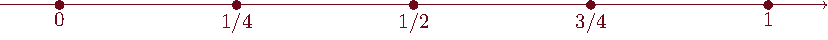
\includegraphics[]{"./proofs/fig1.pdf"}
    \caption{Le découpage pour \(a = 0\), \(b = 1\), \mintinline{cpp}{steps} = 4}
\end{figure}

\theoreme{}\\
\mintinline{cpp}{HistogramMethod} est \(\varepsilon\)-\textit{differentially private}.\\


\textit{Démonstration:} Les requêtes envoyé par l'algorithme à \mintinline{cpp}{AboveThreshold} sont bien de sensibilité 1. Chacun des neuf appels à cette fonction est donc \(\varepsilon/9\)-\textit{differentially private}. Le théorème de composition assure alors que \mintinline{cpp}{HistogramMethod} est \(\varepsilon\)-\textit{differentially private}.\\

Maintenant que nous avons vu que cet algorithme est bien \textit{differentially private}, nous allons essayer d'évaluer sa précision. Cela ne sera pas évident car la précision de l'algorithme dépend beaucoup du jeu de donné en entré.\\




\lemme{\mintinline{cpp}{AboveThreshold} est \((\alpha, \beta)-accurate\)} \label{ATalphabeta}\\
Pour tout \(\beta \in ]0,1[\), tout \(x \in \mathcal X^{(\N)}\), tout \(\{f_i\}_i = Q \in \left( \mathcal X^{(\N)} \to  \mathcal T \right)^{\N}\), tout \(\varepsilon > 0\), tout \(T \in \R\),  en posant \(\alpha = 8\left( \log(k) + \log(2/\beta) \right)/\varepsilon\) et \(k = \) \mintinline{cpp}{AboveThreshold(x, Q, T, epsilon)}, on a, en reprenant les notations de l'algorithme,
\[
    \mathbb P \left( \forall i < k \  f_i(x) + \nu_i < T + \alpha \wedge f_k(x) + \nu_k > T - \alpha \right) \geq 1 - \beta
\]

\textit{\textbf{Remarque:} Ce lemme est due à \cite[page 61]{dwork2014the}. Nous reprenons aussi la démonstration ici car la démonstration originale ne nous semble pas assez claire et trop bancale mathématiquement.}\\

\textit{Démonstration:} Reprenons les notations de l'énoncé. Montrons déjà qu'il suffit de démontrer que 
\begin{align}
    \label{accu_lemme}
    \mathbb P\left( \max_{i \leq k} |\nu_i| + |T - \hat T| < \alpha  \right)  \geq 1 - \beta   
\end{align}
où \(\hat T\) est le seuil bruité défini à la ligne 4 de l'algorithme [\ref{AboveThreshold}]. Or, nous avons, en posant pour tout \(i \leq k\), \(y_i = f_i(x)\)
\[
    y_k + \nu_k \geq \hat T \overset{\text{IT}}{\geq} T - |T-\hat T|
\]

\textit{Mutatis mutandis} 
\[
    \forall i < k \quad y_i \leq \hat T + |\nu_i| \leq T + |T - \hat T| + |\nu_i|  
\]

Ainsi,
\[
    \mathbb P \left( \forall i < k \  f_i(x) + \nu_i < T + \alpha \wedge f_k(x) + \nu_k > T - \alpha \right) \geq 1 - \beta
\]

\textit{Démontrons enfin (\ref{accu_lemme})}! La variable aléatoire \(T-\hat T\) suit une loi de {\sc Laplace} de paramètre \(2/\varepsilon\). Ainsi,
\[
    \mathbb P \left( |T - \hat T| \geq \dfrac{\alpha}{2} = \dfrac{\alpha \varepsilon}{4}\dfrac{2}{\varepsilon} \right) = \exp\left( -\dfrac{\varepsilon \alpha}{4} \right) = \exp\left( -2\left( \log k + \log \dfrac{2}{\beta} \right) \right) \leq \exp\left( -2\left(\log \dfrac{2}{\beta} \right) \right) \leq \dfrac{\beta}{2}
\]

De même,
\[
    \mathbb P \left( \max_{i} |\nu_i| \geq \dfrac{\alpha}{2} \right) \leq \sum\limits_{j = 1}^k \mathbb P \left( |\nu_j| \geq \dfrac{\alpha}{2} \right) = k \exp\left( -\dfrac{-\alpha\varepsilon}{8} \right) = k \exp\left( -\log k - \log\dfrac{2}{\beta} \right) = \dfrac{k}{k} \dfrac{\beta}{2}
\]

Enfin, 
\begin{align*}
    \mathbb P\left( \max_{i \leq k} |\nu_i| + |T - \hat T| < \alpha  \right) & \geq \mathbb P\left( \max_{i \leq k} |\nu_i| < \dfrac{\alpha}{2} \ \wedge \ |T - \hat T| < \dfrac{\alpha}{2} \right)\\
    & = 1 - \mathbb P\left( \max_{i \leq k} |\nu_i| \geq \dfrac{\alpha}{2} \ \cup \ |T - \hat T| \geq \dfrac{\alpha}{2} \right)\\
    & \geq 1 - \mathbb P\left( \max_{i \leq k} |\nu_i| \geq \dfrac{\alpha}{2}\right) - \mathbb P \left(|T - \hat T| \geq \dfrac{\alpha}{2} \right)\\
    &\geq 1 - \dfrac{\beta}{2} - \dfrac{\beta}{2}
\end{align*}

Finalement, 
\[
    \mathbb P\left( \max_{i \leq k} |\nu_i| + |T - \hat T| < \alpha  \right)  \geq 1 - \beta
\]

Ce qui démontre bien (\ref{accu_lemme}) et donc le lemme.\\

\subsection{Analyse de complexité}

La complexité de \mintinline{cpp}{AboveThreshold} est de l'ordre de la somme des complexité des requêtes sur le jeu de données d'entré. En notant \(n\) la taille de la base de donnée, les requêtes envoyé à \mintinline{cpp}{AboveThreshold} par \mintinline{cpp}{HistogramMethod} sont toute de complexité linéaire en \(n\). Il y a au plus \(\O(n/\log n)\) requêtes envoyées. L'algorithme a alors une complexité en \(\O(n^2/\log n)\).

\subsection{Analyse de précision - le cas de la distribution uniforme standard}

Nous allons évaluer la précision de l'algorithme à l'aide de l'erreur quadratique moyenne entre la valeur renvoyé par le programme et la valeur attendue. Il y a plusieurs manière de penser ce qu'est la valeur attendue: elle pourrait être la valeur des déciles de l'échantillons d'entré. Néanmoins, elle peut tout aussi bien être l'ensemble des déciles de la loi. En effet, nous cherchons à répondre à des questions de statistique, l'entré peut-être un simple échantillon ``représentatif'';  au quel cas nous sommes principalement intéressé par les réponses statistiques sur l'ensemble de la population et non juste sur notre échantillon.\\

Ces deux choix ont un réel sens. Nous avons d'abord essayé d'évaluer les performances de l'algorithme dans le premier cas. Les calculs était difficiles et menaient à des résultats difficilement exploitables. Nous avons donc choisi de réaliser les calculs sur la seconde option afin de pouvoir mener des calculs légèrement plus simples et ainsi avoir des résultats.\\

\subsubsection{Analyse de précision: borne exacte}

Nous allons commencer par démontrer quelques lemmes intermédiaires afin de démontrer les résultats de précision. Mais d'abord, donnons les définitions qui nous serrons utiles ici.\\

\definition{Fonction Beta incomplète}\\
On appel fonction beta incomplète la fonction 
\[
    B : \left\{ 
        \begin{array}[]{ccc}
            [0,1] \times (\R_+^\star)^2 & \to & \R_+\\
            (x, \alpha, \beta) & \mapsto & \displaystyle\int_0^x t^{\alpha - 1} (1 - t)^{\beta -1} \dt t
        \end{array}
    \right.    
\]

\definition{Fonction Beta incomplète régularisée }\\
Pour tout \(x \in [0,1]\), on appel fonction beta incomplète régularisée la fonction 
\[
    I_x : \left\{ 
        \begin{array}[]{ccc}
            (\R_+^\star)^2 & \to & \R_+\\
            (\alpha, \beta) & \mapsto & \dfrac{B(x, \alpha, \beta)}{B(1, \alpha, \beta)}
        \end{array}
    \right.    
\]

\definition{Loi beta}\\
On appel loi beta de paramètre \((\alpha, \beta) \in \R_+^\star\) la loi de densité
\[
        f_{\alpha,\beta} : [0,1] \ni x \mapsto \dfrac{x^{\alpha - 1} (1-x)^{\beta} - 1}{B(1, \alpha, \beta)}
\]

\textbf{Remarque:} \textit{On note directement que la fonction de répartition de la loi beta de paramètre \((\alpha, \beta)\) est la fonction \(x \mapsto I_x(\alpha, \beta)\).}\\

\definition{Statistique d'ordre}\\
Soit \(X\) un échantillon statistique de cardinal \(n \in \N\). Pour tout \(k \in \inte 1 n \) on note \(X_{(i)}\) et on appel \textbf{statistique d'ordre} de rang \(k\) la \(k\)-ème plus petite valeur de l'échantillon.\\


\theoreme{Loi des statistiques d'ordre d'un échantillon issue de \(\mathcal U(0,1)\).}\label{staorduni}\\
Soit \(X\) un ensemble de \(n\) variables aléatoires \((X_i)_i\) indépendantes et suivant toutes la loi uniforme sur [0,1] et \(k \in \inte 1 n \). La \(k\)-ème statistique d'ordre de \(X\), \(X_{(k)}\) est distribuée suivant la loi beta de paramètre \((k, n-k+1)\).\\

\textit{Démonstration:} disponible en annexe [\ref{statordre}]. \\



\lemme{Estimation de l'écard entre certaines statistiques d'ordre et les déciles.}\\
Soit \(X\) un ensemble de \(n\) variables aléatoires \((X_i)_i\) indépendantes et suivant toutes la loi uniforme sur [0,1], \(\gamma \in [0, d_i^l]\) et \(\alpha \in [0, n/10]\). Notons \((d_i^l)_i\) les déciles de la loi. Pour tout \(i \in \inte 1 9\)
\begin{align*}
    \mathbb P \left( [X_{(in/10 - \alpha)}, X_{(in/10 + \alpha)}] \subset [d_i^l - \gamma, d_i^l + \gamma] \right) \geq & I_{d_i^l + \gamma}(in/10 + \alpha, n - in/10 -  \alpha + 1)\\
    &\quad - I_{d_i^l - \gamma}(in/10 - \alpha, n - in/10 +  \alpha + 1)
\end{align*}

\textit{Démonstration:} Notons que 
\begin{align*}
    \mathbb P \left( [X_{(in/10 - \alpha)}, X_{(in/10 + \alpha)}] \subset [d_i^l - \gamma, d_i^l + \gamma] \right) & = \mathbb P (X_{(in/10 - \alpha)} \geq d_i^l - \gamma \ \wedge \ X_{(in/10 + \alpha)} \leq d_i^l + \gamma )\\
    & \geq \mathbb P(X_{(in/10 - \alpha)} \geq d_i^l - \gamma) + \mathbb P(X_{(in/10 + \alpha)} \leq d_i^l + \gamma) - 1
\end{align*}

Or, le théorème précédent assure que 
\[
    \left\{
        \begin{array}[]{rcl}
            \mathbb P(X_{(in/10 - \alpha)} \geq d_i^l - \gamma) & = & 1 - I_{d_i^l - \gamma}(in/10 - \alpha, n - in/10 +  \alpha + 1)\\
            \mathbb P(X_{(in/10 + \alpha)} \leq d_i^l + \gamma) & = & I_{d_i^l + \gamma}(in/10 + \alpha, n - in/10 -  \alpha + 1)\\
        \end{array}
    \right.
\]

D'où
\begin{align*}
    \mathbb P \left( [X_{(in/10 - \alpha)}, X_{(in/10 + \alpha)}] \subset [d_i^l - \gamma, d_i^l + \gamma] \right) \geq & I_{d_i^l + \gamma}(in/10 + \alpha, n - in/10 -  \alpha + 1)\\
    &\quad - I_{d_i^l - \gamma}(in/10 - \alpha, n - in/10 +  \alpha + 1)
\end{align*}

% \textit{Démonstration:} Soit \(X\) un ensemble de \(n\) variables aléatoires \((X_i)_i\) indépendantes et suivant toutes la loi uniforme sur [0,1]. Notons \((d_i)_i\) les déciles empiriques de \(X\) et \((d_i^l)_i\) ceux de la loi. Soit \(\gamma \in [0,2d_i^l]\). On note que
% \[
%         d_i = X_{(in/10)} 
% \]

% Le théorème [\ref{staorduni}] assure alors que 
% \[
%     \mathbb P(d_i \in [d_i^l - \gamma/2, d_i^l + \gamma/2]) = I_{d_i^l + \gamma/2}(in/10, (10-i)n/10 +1) - I_{d_i^l - \gamma/2}(in/10, (10-i)n/10 +1)
% \]


% % \begin{align*}
% %     \mathbb P(d_i \in [d_i^l - \gamma/2, d_i^l + \gamma/2]) & = 1 - \mathbb P(d_i \notin [d_i^l - \gamma/2, d_i^l + \gamma/2])\\
% %     & = 1 - \mathbb P(d_i \leq d_i^l - \gamma/2 \vee d_i \geq d_i^l + \gamma/2])
% % \end{align*}

% % On pose alors \(A = \) ``il y a au moins \(in/10\) valeurs plus petites que \(d_i^l - \gamma/2\)'' et \(B = \) ``il y a au plus \(in/10\) valeurs plus petites que \(d_i^l + \gamma/2\)''. On pose donc pour tout \(j\), \(A_j = \un_{x_j < d_i^l - \gamma/2}\) et \(B_j = \un_{x_j < d_i^l + \gamma/2}\).  On pose alors \(A_s = \sum_{j = 0}^{n-1} A_j\) et \(B_s = \sum_{j = 0}^{n-1} B_j\)

% % \begin{align*}
% %     \mathbb P(d_i \in [d_i^l - \gamma/2, d_i^l + \gamma/2]) & = 1 - \mathbb P(A \cup B)\\
% %     & \geq 1 - \mathbb P(A) - \mathbb P(B)\\
% %     & \geq 1 - \mathbb P(A_s \geq in/10) - \mathbb P(B_s \leq in/10)\\
% % \end{align*}

% % Les événements \((A_j)_j\) suivent une loi de {\sc Bernouilli} de paramètre \(d_i^l - \gamma/2\) et les événements \((B_j)_j\) suivent une loi de {\sc Bernouilli} de paramètre \(d_i^l + \gamma/2\). Ainsi, 
% % \[
% %     \begin{array}{rcl}
% %         \mathbb P \left( A_s \geq in/10 \right) & \overset{d_i^l = i/10}{=} & \mathbb P \left( A_s \geq \left( d_i^l - \dfrac{\gamma}{2} \right)n\left(1 +\left(\dfrac{d_i^l}{d_i^l - \gamma/2} - 1 \right)\right)\right)\\
% %         & \leq & \exp\left( -\dfrac{1}{3}n\left( d_i^l - \dfrac{\gamma}{2} \right) \left(\dfrac{\gamma/2}{d_i^l - \gamma/2} \right)^2 \right)\\
% %         & = & \exp\left( -\dfrac{1}{12}n\gamma^2 \dfrac{1}{d_i^l - {\gamma}/{2}} \right)\\
% %         & \overset{d_i^l - \gamma/2 \leq 1}{\leq} & \exp\left( -\dfrac{1}{12}n\gamma^2 \right)\\
% %     \end{array}
% % \]

% % De même
% % \[
% %     \mathbb P\left( B_s \leq \dfrac{in}{10} \right) \leq \exp\left( -\dfrac{1}{12}n\gamma^2 \right)
% % \]

% % Finalement,
% % \[
% %     \mathbb P(d_i \in [d_i^l - \gamma/2, d_i^l + \gamma/2]) \geq 1 - 2\exp\left( -\dfrac{1}{12}n\gamma^2 \right)\\
% % \]


% \lemme{}

% Soit \(X\) un ensemble de \(n\) variables aléatoires \((X_i)_i\) indépendantes et suivant toutes la loi uniforme sur [0,1] dont on note \((d_i^l)_i\) les déciles. Soit \(\gamma \in [0,2d_i^l]\), \(i \in \inte 1 9 \) et \(\alpha \in [0, \gamma n /2[\). Il y a au moins \(\alpha\) valeurs de \(X\) dans chacun des intervalles \([d_i^l - \gamma, d_i^l-\gamma/2]\) et \([d_i^l + \gamma/2, d_i^l+\gamma]\) avec une probabilité au moins \(1 - \beta\) avec 
% \[
%     \beta = 2\exp\left( - \dfrac{n\gamma^2}{2}\left(1 - \dfrac{2\alpha}{n\gamma}\right)^2\right)
% \]

% \textit{Démonstration:} Soit \(X\) un ensemble de \(n\) variables aléatoires \((X_i)_i\) indépendantes et suivant toutes la loi uniforme sur [0,1] dont on note \((d_i^l)_i\) les déciles. Soit \(\gamma \in [0,2d_i^l]\), \(i \in \inte 1 9 \) et \(\alpha \in [0, \gamma n /2[\). On pose alors pour tout \(j\), \(A_j = \un_{x_j \in d_i^l - \gamma, d_i^l - \gamma/2}\) et \(B_j = \un_{x_j \in d_i^l + \gamma/2, d_i^l + \gamma}\). On peut alors noter \(A = \sum_{j = 0}^{n-1} A_j\) et  \(B = \sum_{j = 0}^{n-1} B_j\). 
% \begin{align*}
%     \mathbb P \left( A \geq \alpha \ \wedge \ B \geq \alpha \right) & \geq \mathbb P (A \geq \alpha) + \mathbb P (B \geq \alpha) - 1
% \end{align*}

% Or, on a, à l'aide de l'inégalité d'{\sc H\oe ffding}\footnote{Nous avions initialement utilisé l'inégalité de {\sc Chernoff}. Néanmoins cette inégalité permet une légère amélioration qui fera une différence notable après intégration pour l'estimation de l’espérance.},
% \[
%     \left\{
%     \begin{array}{rcl}
%         \mathbb P (A \geq \alpha) & = & 1 - \mathbb P \left(A < \dfrac{n\gamma}{2}\left(1 -\left(1 - \dfrac{2\alpha}{n\gamma}\right)\right)\right) \overset{\alpha < \gamma n /2}{\geq} 1 - \exp\left( - 2\dfrac{n^2\gamma^2}{2^2n}\left(1 - \dfrac{2\alpha}{n\gamma}\right)^2\right)\\
%         \mathbb P (B \geq \alpha) & = & 1 - \mathbb P \left(B < \dfrac{n\gamma}{2}\left(1 -\left(1 - \dfrac{2\alpha}{n\gamma}\right)\right)\right) \overset{\alpha < \gamma n /2}{\geq} 1 - \exp\left( - 2\dfrac{n^2\gamma^2}{2^2n}\left(1 - \dfrac{2\alpha}{n\gamma}\right)^2\right)\\
%     \end{array}
%     \right.
% \]

% Ainsi,
% \begin{align*}
%     \mathbb P \left( A \geq \alpha \ \wedge \ B \geq \alpha \right) & \geq 1 - 2\exp\left( - \dfrac{n\gamma^2}{2}\left(1 - \dfrac{2\alpha}{n\gamma}\right)^2\right)
% \end{align*}


La combinaison des lemmes précédents permet d'obtenir un résultat de précision utile sur \mintinline{cpp}{HistogramMethod}.\\


\theoreme{\((\alpha, \beta)\)-précision de \mintinline{cpp}{HistogramMethod} dans le cas uniforme standard}

Soit \(X\) un ensemble de \(n\) (tel que \(0\leq 8\log(3n/(\beta\log n))/\varepsilon) \leq n/10\)) variables aléatoires \((X_i)_i\) indépendantes et suivant toutes la loi uniforme sur [0,1]. Soit \(\gamma \in [0,d_i^l]\), \(i \in \inte 1 9 \) et \(\beta \in [0,1]\). Notons \((d_i^l)_i\) les déciles de la loi. Posons \(A\) la variable aléatoire \mintinline{cpp}{HistogramMethod(X, epsilon, 0, 1)}, \(\alpha = 8\log(3n/(\beta\log n))/\varepsilon)\) et \( k = 1.5n/\log n\).

\begin{align*}
    \mathbb P\left( A_i \in \left[d_i^l-\gamma - \dfrac{1}{k}, d_i^l + \gamma + \dfrac{1}{k} \right] \right) & \geq   I_{d_i^l + \gamma}(in/10 + \alpha, n - in/10 -  \alpha + 1)\\
    &\quad - I_{d_i^l - \gamma}(in/10 - \alpha, n - in/10 +  \alpha + 1) - \beta
\end{align*}



\textit{Démonstration:} Notons \(E_\alpha\) l'événement ``\( [X_{(in/10 - \alpha)}, X_{(in/10 + \alpha)}] \subset [d_i^l - \gamma, d_i^l + \gamma]\)'' Et \(E_{A_i}\) l'événement ``moins de \(\alpha\) valeurs de \(X\) séparent \(d_i\) et une valeur de \(X\) dont la distance à \(A_i\) est majorée par \(1/k\)''. Nous avons alors 
\begin{align*}
    \mathbb P\left( A_i \in \left[d_i^l-\gamma - \dfrac{1}{k}, d_i^l + \gamma + \dfrac{1}{k}\right] \right) & \geq \mathbb P \left( E_{A_i} \wedge E_\alpha  \right) \geq \mathbb P \left( E_{A_i}\right) + \mathbb P \left( E_\alpha\right) - 1
\end{align*}

Le lemme [\ref{ATalphabeta}] assure que 
\[
    \mathbb P (E_{A_i}) \geq 1 - \beta 
\]

En effet, ce lemme assure que si la réponse renvoyée ne dépassait pas le seuil, l'évaluation de la requête valait au moins \(T - \alpha\) (en notant \(T\) le seuil) avec une probabilité minorée par \(1 - \beta\). De plus, avec cette même probabilité, on sait que l'évaluation de l'avant dernière requête était majorée par \(T +\alpha\) (toujours en notant \(T\) le seuil). Ainsi, comme \(T = in/10\), \(E_{A_i}\) est de probabilité au moins \(1 - \beta\).\\

Le lemme précédent assure alors que 
\begin{align*}
    \mathbb P\left( A_i \in \left[d_i^l-\gamma - \dfrac{1}{k}, d_i^l + \gamma + \dfrac{1}{k} \right] \right) & \geq   I_{d_i^l + \gamma}(in/10 + \alpha, n - in/10 -  \alpha + 1)\\
    &\quad - I_{d_i^l - \gamma}(in/10 - \alpha, n - in/10 +  \alpha + 1) - \beta
\end{align*}



Ce résultat n'est pas optimal. Nous avons fait des approximations. Néanmoins, nous avons une bonne borne. Nous allons maintenant utiliser ce théorème pour obtenir un résultat très important: une majoration de l’espérance de la distance entre la valeur renvoyée par le mécanisme et un décile de la loi. Ce résultat permet de savoir quelle est l'erreur à laquelle s'attendre en pratique. \\

\theoreme{Précision moyenne de \mintinline{cpp}{HistogramMethod}}
Soit \(X\) un ensemble de \(n\) (tel que \(0\leq 8\log(3n/(\beta\log n))/\varepsilon) \leq n/10\)) variables aléatoires \((X_i)_i\) indépendantes et suivant toutes la loi uniforme sur [0,1]. Soit \(i \in \inte 1 9 \), \(k \in \N\) et \(\beta \in [0,1]\). Notons \((d_i)_i\) les décile de la loi. Posons \(A\) la variable aléatoire  \mintinline{cpp}{HistogramMethod(X, epsilon, 0, 1)} et \(\alpha = 8\log(3n/(\beta\log n))/\varepsilon)\)\\
\begin{align*}
    \mathbb E\left( |A_i - d_i^l| \right) & \leq  \dfrac{2\log n}{3n} + d_i^l\beta + \int_{0}^{d_i^l}\left( 1 - I_{d_i^l + t}(in/10 + \alpha, n - in/10 -  \alpha + 1) \right) \dt t\\
    &\quad + \int_{0}^{d_i^l}I_{d_i^l - t}(in/10 - \alpha, n - in/10 +  \alpha + 1) \dt t\\
    &\quad + \left(1 - d_i^l - \dfrac{2\log n}{3n}\right)\left(1 + \beta -  I_{2d_i^l}(in/10 + \alpha, n - in/10 -  \alpha + 1) \right)
\end{align*}

\textit{Démonstration:} On pose 
\[
    F : \left\{
        \begin{array}[]{ccc}
            \R_+ & \to & [0,1]\\
            t & \mapsto & \mathbb P(|A_i - d_i^l| \leq t)
        \end{array}
    \right.   
\]

Le théorème précédent assure que 
\begin{align*}
    \forall t \in [0, 2d_i^l] \quad F\left( t + \dfrac{1}{k} \right) & := \mathbb P\left(|A_i - d_i^l| \leq t + \dfrac{1}{k}\right) \\
    & \geq  I_{d_i^l + t}(in/10 + \alpha, n - in/10 -  \alpha + 1)\\
    & \quad - I_{d_i^l - t}(in/10 - \alpha, n - in/10 +  \alpha + 1) - \beta
\end{align*}

% Notons aussi grâce aux propriétés de base sur les fonctions de répartition que
% \[
%     \left\{
%        \begin{array}[]{ll}
%             \forall t \leq 1/k \quad F(t) \leq 1\\
%             \forall t \geq 1/k + d_i^l \quad F(t) \geq F\left( \dfrac{1}{k} + d_i^l \right) \geq 1 - 2k\exp\left(- \dfrac{\varepsilon d_i^l}{24}n \right) - 4\exp\left( - \dfrac{(d_i^l)^2}{18}n\right)
%        \end{array} 
%     \right.
% \]

Or, comme \(F(1) = 1\),
\[
    \mathbb E\left( |A_i - d_i^l| \right) = \int_0^{\infty} (1 - F(t))\dt t = \int_{0}^{1/k} (1 - F(t))\dt t + \int_{1/k}^{d_i^l + 1/k} (1 - F(t))\dt t + \int_{d_i^l + 1/k}^{1} (1 - F(t))\dt t
\]

Notons que 
\[
    \int_0^{1/k} (1 - F(t))\dt t \leq \int_0^{1/k}\dt t = \dfrac{1}{k}
\]

% Mais aussi que
% \[
%     \int_{1/k}^{d_i^l + 1/k} (1 - F(t))\dt t = d_i^l  - \int_{1/k}^{d_i^l + 1/k} F(t)\dt t \leq 
% \]

% Or,
% \[
%     \int_{1/k}^{d_i^l + 1/k} 2k\exp\left(- \dfrac{\varepsilon t}{24}n \right) \dt t \leq \int_{0}^{d_i^l + 1/k} 2k\exp\left(- \dfrac{\varepsilon t}{24}n \right) \dt t \leq \dfrac{48k}{\varepsilon n} 
% \]
% \begin{align*}
%     \\
%     % & = \int_{1/k}^{d_i^l} (1 - F(t))\dt t + 0 + \int_{0}^{1/k} (1 - F(t))\dt t\\
%     &\leq \dfrac{1}{k} + \int_{0}^{d_i^l} \left( 2k\exp\left(- \dfrac{\varepsilon t}{24}n \right) + 4\exp\left( - \dfrac{t^2}{18}n\right)  \right)\dt t\\
%     & \quad   + \left( 1 - d_i^l - \dfrac{1}{k} \right)\left( 2k\exp\left(- \dfrac{\varepsilon d_i^l}{24}n \right) + 4\exp\left( - \dfrac{(d_i^l)^2}{18}n\right) \right)
% \end{align*}

Or, les propriétés usuelles sur les fonctions de répartition assurent que 
\[
    \forall t \geq d_i^l \quad 1 - F(t) \leq 1 - F(d_i^l)
\]

Ainsi,
\[
    \int_{d_i^l + 1/k}^{1} (1 - F(t))\dt t \leq \left(1 - d_i^l - \dfrac{1}{k}\right)\left(1 + \beta -  I_{2d_i^l}(in/10 + \alpha, n - in/10 -  \alpha + 1) \right)
\]

% De plus,
% \[
%     \int_{0}^{d_i^l} 4\exp\left( - \dfrac{t^2}{18}n\right) \dt t \leq 4\int_{\R_+} \exp\left( - \dfrac{t^2}{18}n\right) \dt t = \dfrac{12\sqrt{2}}{\sqrt{n}}\int_{\R_+} \exp\left( - t^2\right) \dt t \leq 12\sqrt{\dfrac{2\pi}{n}}
% \]

Finalement, nous avons démontré que 
\begin{align*}
    \mathbb E\left( |A_i - d_i^l| \right) & \leq  \dfrac{1}{k} + d_i^l\beta + \int_{0}^{d_i^l}\left( 1 - I_{d_i^l + t}(in/10 + \alpha, n - in/10 -  \alpha + 1) \right) \dt t\\
    &\quad + \int_{0}^{d_i^l}I_{d_i^l - t}(in/10 - \alpha, n - in/10 +  \alpha + 1) \dt t\\
    &\quad + \left(1 - d_i^l - \dfrac{1}{k}\right)\left(1 + \beta -  I_{2d_i^l}(in/10 + \alpha, n - in/10 -  \alpha + 1) \right)
\end{align*}

Ce résultat est vrai pour toutes valeurs de \(\beta\). Nous pourrions donc majorer notre espérance par une borne inférieure. Néanmoins cela n'aurait aucun sens ici: assez d'approximations ont étés faites pour qu'une utiliser un résultat ``exacte'' soit futile; une borne inf est jolie sur le papier mais n'est en pratique que difficilement exploitable. Des calculs numériques montrent que le choix \(\beta = 1/(\sqrt n \log n )\) n'est ``pas trop'' éloignée de cette borne inf. Nous disposons alors du corollaire suivant.\\

\coro{(im)Précision moyenne de \mintinline{cpp}{HistogramMethod}}\label{coro_err_quadra}
Soit \(X\) un ensemble de \(n\) (tel que \(0\leq 8\log(3n\sqrt n)/\varepsilon) \leq n/10\)) variables aléatoires \((X_i)_i\) indépendantes et suivant toutes la loi uniforme sur [0,1]. Soit \(i \in \inte 1 9 \) et \(k \in \N\). Notons \((d_i)_i\) les décile de la loi. Posons \(A\) la variable aléatoire  \mintinline{cpp}{HistogramMethod(X, epsilon, 0, 1)} et \(\alpha = 8\log(3n\sqrt n)/\varepsilon)\).\\

\begin{align*}
    \mathbb E\left( |A_i - d_i^l| \right) & \leq  \dfrac{2\log n}{3n} + \dfrac{d_i^l}{\sqrt n \log n} + \int_{0}^{d_i^l}\left( 1 - I_{d_i^l + t}(in/10 + \alpha, n - in/10 -  \alpha + 1) \right) \dt t\\
    &\quad + \int_{0}^{d_i^l}I_{d_i^l - t}(in/10 - \alpha, n - in/10 +  \alpha + 1) \dt t\\
    &\quad + \left(1 - d_i^l - \dfrac{2\log n}{3n}\right)\left(1 + \dfrac{1}{\sqrt n \log n} -  I_{2d_i^l}(in/10 + \alpha, n - in/10 -  \alpha + 1) \right)
\end{align*}


\begin{figure}[H]
    \centering
    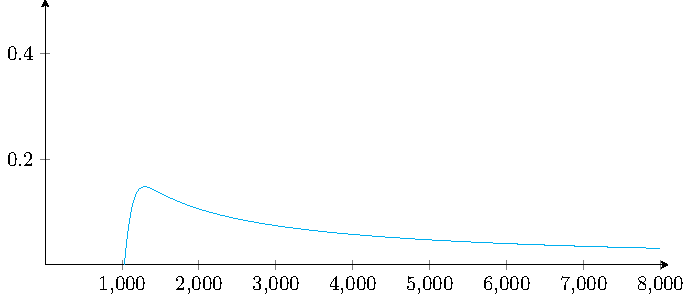
\includegraphics[]{"./proofs/fig5.pdf"}
    \caption{Graphe de la borne du corollaire [\ref{coro_err_quadra}] en fonction de \(n\) avec \(\varepsilon = 1\).}
\end{figure}
% \begin{figure}[H]
%     \centering
%     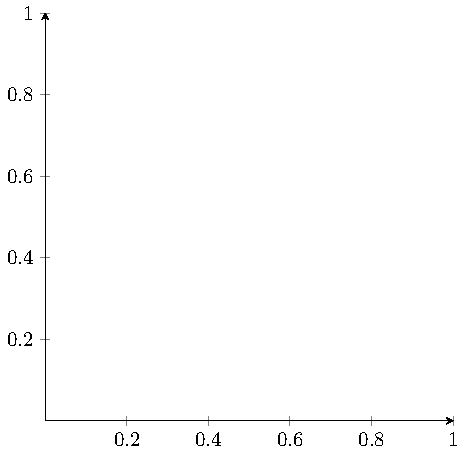
\includegraphics[width=0.3\textwidth]{"./proofs/fig0.pdf"}
%     \caption{Graphes de \(\color{magenta}\beta \mapsto \dfrac{1}{k} + \left(d_i^l - \dfrac{1}{k}\right)\beta + 2\sqrt \dfrac{3\pi}{n} + \dfrac{4\sqrt{\pi}}{\sqrt{n - 4\alpha}}e^{-\alpha^2}\) pour \(i = 5\), \(n = 10000\), \(k = 100\) et \(\varepsilon = 1\)}
%     \label{fig:mygraph}
% \end{figure}

\subsubsection{Analyse de précision: borne asymptotique}

Le calcul d'une borne asymptotique sur l'espérance de la distance entre la sortie de l'algorithme et les déciles de la loi est obtenue à partir d'une majoration asymptotique du résultat du corollaire précédent [\ref{coro_err_quadra}]. Obtenir cette borne n'a pas été facile, il a fallut effectuer de nombreux essaies avant de trouver une solution convenable: beaucoup de méthodes ne permettent pas une bonne simplification et fait alors obtenir une borne qui tend vers \(+\infty\), une borne inutile! Cette sous-sous-section présente le résultat que nous avons finalement réussis à obtenir.\\

Soit \(X\) un ensemble de \(n\) (tel que \(0\leq 8\log(3n\sqrt n)/\varepsilon) \leq n/20\)) variables aléatoires \((X_i)_i\) indépendantes et suivant toutes la loi uniforme sur [0,1]. Soit \(i \in \inte 1 9 \) et \(k \in \N\). Notons \((d_i)_i\) les décile de la loi. Posons \(A\) la variable aléatoire  \mintinline{cpp}{HistogramMethod(X, epsilon, 0, 1)} et \(\alpha = 8\log(3n\sqrt n)/\varepsilon)\).\\

% Afin de pouvoir appliquer les inégalité qui nous intéressent, il nous faut \(\log(3n\sqrt n ) \leq \dfrac{nt\varepsilon}{8}\). Nous reviendront sur cette borne plus tard. Cette borne donne une minoration sur les valeurs de \(n\) pour lesquelles la majoration est valide.\\

Nous allons commencer par majorer le terme suivant: 
\[
    \int_{0}^{d_i^l}\left( 1 - I_{d_i^l + t}(in/10 + \alpha, n - in/10 -  \alpha + 1) \right) \dt t    
\]

Soit \(t \in [0, d_i^l]\). Notons que 
\[
    \begin{array}[]{rcl}
        1 - I_{d_i^l + t}(in/10 + \alpha, n - in/10 -  \alpha + 1) & = & I_{1 - (d_i^l + t)}(n - (in/10 + \alpha - 1), (in/10 + \alpha - 1) + 1)\\
        & \overset{\text{déf}}{:=} & I_{1 - p}(n - k, k + 1)  
    \end{array}  
\]

Or, si \(X\) suit une loi binomial de paramètres \(n,p\), \(I_{1 - p}(n - k, k + 1)  = \mathbb P(X \leq k)\). Nous souhaitons appliquer une application de l'inégalité d'{\sc Hoeffding} (démontré en annexe [\ref{hoef}]). Pour cela il nous faut \(k \leq np\). Il suffit pour cela que nous ayons \(\alpha \leq nt\). Se restreindre aux \(t \geq 12\log(3^{2/3}n)/(n\varepsilon)\) permet donc d'appliquer l'inégalité.
\begin{align*}
    1 - I_{d_i^l + t}(in/10 + \alpha, n - in/10 -  \alpha + 1) & \leq \exp\left( -2n\left( p - \dfrac{k}{n} \right)^2 \right)\\
    & = \exp\left( - 2\dfrac{k^2}{n} \right)\exp\left( -2np^2 + 4pk \right)
\end{align*}

De plus,
\begin{align*}
    \int_0^{d_i^l}\exp\left( -2np^2 + 4pk \right)\dt & = \int_{d_i^l}^{{2d_i^l}}\exp\left( -2nt^2 + 4tk \right)\dt t \\
    & \leq \int_{\R}\exp\left( -2nt^2 + 4tk \right)\dt t \\
    & = \int_{\R}\exp\left( -2n\left(t - \dfrac{k}{n}\right)^2 + 2 \dfrac{k^2}{n} \right)\dt t \\
    & = \dfrac{1}{\sqrt{2n}}\exp\left( 2 \dfrac{k^2}{n} \right) \int_{\R}\exp\left( -t^2 \right)\dt t \\
    & = \sqrt{\dfrac{\pi}{2n}}\exp\left( 2 \dfrac{k^2}{n} \right)\\
\end{align*}

Nous avons donc montré que,
\begin{align}
    \int_{0}^{d_i^l}\left( 1 - I_{d_i^l + t}(in/10 + \alpha, n - in/10 -  \alpha + 1) \right) \dt t \leq \dfrac{12}{n\varepsilon}\log(3^{2/3}n) + \sqrt{\dfrac{\pi}{2n}}
\end{align}

Nous pouvons alors entamer la majoration du terme suivant 
\[
    \int_{0}^{d_i^l}I_{d_i^l - t}(in/10 - \alpha, n - in/10 +  \alpha + 1) \dt t    
\]

Soit \(t \in [0, d_i^l]\). Notons que 
\[
    \begin{array}[]{rcl}
        I_{d_i^l - t}(in/10 - \alpha, n - in/10 +  \alpha + 1) & \overset{\text{déf}}{:=} & I_{p}(k+1, n - k)\\
        & = & \mathbb P(X > k)
    \end{array}    
\]

Où \(X\) suit une loi binomiale de paramètre \((n,p)\). Nous souhaitons une nouvelle fois appliquer l'inégalité d'{\sc Hoeffding} (démontré en annexe [\ref{hoef}]). Pour cela, il nous faut \(k \geq np\). Il suffit alors d'avoir \(nt \geq \alpha + 1\) donc d'avoir \(t \geq 12\log(3^{2/3}n)/(\varepsilon n) + 1/n\). En se restreignant à ces valeurs de \(t\) nous avons donc 
\begin{align*}
    \mathbb P(X > k) & \leq \exp\left( -2np^2\left( \dfrac{k}{np} - 1 \right)^2 \right)\\
    & = \exp\left(  -2\dfrac{k^2}{n} +4kp  - 2np^2  \right)
\end{align*}

Ainsi,
\begin{align*}
    \int_0^{d_i^l} I_{p}(k+1, n - k) \dt t & = \int_{0}^{d_i^l} I_{t}(k+1, n - k) \dt t \\
    & \leq \exp\left( -2\dfrac{k^2}{n} \right) \int_\R \exp\left( -2np^2 + 4kp \right)\dt t\\
    & = \exp\left( -2\dfrac{k^2}{n} \right) \int_\R \exp\left( -2n\left( p - \dfrac{k}{n} \right)^2 + \dfrac{2k^2}{n} \right)\dt t\\
    & = \sqrt{\dfrac{\pi}{2n}}
\end{align*}

Enfin, nous avons démontré que,
\begin{align}
    \int_{0}^{d_i^l}I_{d_i^l - t}(in/10 - \alpha, n - in/10 +  \alpha + 1) \dt t & \leq \dfrac{12}{\varepsilon n}\log(3^{2/3}n) + \dfrac{1}{n} + \sqrt{\dfrac{\pi}{2n}}
\end{align}

Il ne reste alors plus qu'à majorer le terme suivant
\[
    1 -  I_{2d_i^l}(in/10 + \alpha, n - in/10 -  \alpha + 1)    
\]

Ainsi,
\[
    \begin{array}{rcl}
        1 -  I_{2d_i^l}(in/10 + \alpha, n - in/10 -  \alpha + 1)  & = & I_{1 - 2d_i^l}(n - (in/10 + \alpha - 1), (in/10 + \alpha - 1) + 1)\\
        & \overset{\text{déf}}{:=} & I_{1 - p}(n - k, k+1)
    \end{array}    
\]

La condition initiale sur \(n\) assure que l'on a \(k \leq np\). Ainsi, l'inégalité d'{\sc Hoeffding} (démontré en annexe [\ref{hoef}]) assure que 
\[
    1 -  I_{2d_i^l}(in/10 + \alpha, n - in/10 -  \alpha + 1) \leq \exp\left( -2n\left( p - \dfrac{k}{n} \right)^2 \right)\\
\]

Or, \(n\) est tel que \(24\log(3^{2/3}n)/(\varepsilon n) \leq n/20\)n \(k/n < 3/2 d_i^l\). Ainsi,
\begin{align}
    1 -  I_{2d_i^l}(in/10 + \alpha, n - in/10 -  \alpha + 1) \leq \exp\left( -\dfrac{n(d_i^l)^2}{2} \right)
\end{align}



\theoreme{(im)Précision moyenne de \mintinline{cpp}{HistogramMethod}}\\
Nous pouvons enfin réunir tous ces résultats intermédiaires et énoncer le théorème.\\
Soit \(X\) un ensemble de \(n\) (tel que \(0\leq 8\log(3n\sqrt n)/\varepsilon) \leq n/20\)) variables aléatoires \((X_i)_i\) indépendantes et suivant toutes la loi uniforme sur [0,1]. Soit \(i \in \inte 1 9 \) et \(k \in \N\). Notons \((d_i)_i\) les décile de la loi. Posons \(A\) la variable aléatoire  \mintinline{cpp}{HistogramMethod(X, epsilon, 0, 1)} et \(\alpha = 8\log(3n\sqrt n)/\varepsilon)\).\\

\begin{align*}
    \mathbb E\left( |A_i - d_i^l| \right) & \leq  \dfrac{2\log n}{3n} + \dfrac{d_i^l}{\sqrt n \log n} + 2\sqrt{\dfrac
    {\pi}{2n}} + \left(1 - d_i^l - \dfrac{2\log n}{3n}\right)\left( \dfrac{1}{\sqrt n \log n}  + \exp\left( -\dfrac{n(d_i^l)^2}{2} \right) \right) + \dfrac{24}{\varepsilon n}\log(3^{2/3}n) + \dfrac{1}{n}
\end{align*}


\coro{(im)Précision moyenne de \mintinline{cpp}{HistogramMethod}}\\
Soit \(X\) un ensemble de \(n\) variables aléatoires \((X_i)_i\) indépendantes et suivant toutes la loi uniforme standard. Soit \(i \in \inte 1 9 \). Notons \((d_i)_i\) les décile de la loi. Posons \(A\) la variable aléatoire  \mintinline{cpp}{HistogramMethod(X, epsilon, 0, 1)}.\\

\begin{align*}
    \mathbb E\left( |A_i - d_i^l| \right) = \underset{n}{\mathcal O}\left(\dfrac{1}{\sqrt{n}}\right)
\end{align*}

\subsubsection{Analyse de précision: résultats expérimentaux}

\subsection{Analyse de précision - le cas de la loi normale centrée réduite}

Les lois normales est très utilisées en statistique notamment car elle permettent de modéliser les phénomènes issues de plusieurs événement aléatoires. Le théorème central limite viens jouer un rôle clé dans la prépondérance de l'utilisation de ces lois. Il semble alors crucial d'étudier la précision de notre algorithme dans le cas où les données d'entré suivent une loi normale.\\

Le théorème de précision est très analogue à celui obtenue dans le cas uniforme. Nous ne détaillons pas ici les lemmes intermédiaires et la démonstration car il s'agit formellement de la même chose. Il est néanmoins nécessaire d'introduire quelques objets usuels en plus car la loi normale est plus complexe que la loi uniforme.\\

\definition{Fonction d'erreur}

On appel fonction d'erreur la fonction suivant:
\[
        \erf: \left\{ 
        \begin{array}[]{rcl}
            \C &\to& \C\\
            z &\mapsto& \dfrac{2}{\sqrt \pi} \displaystyle\int_0^z\exp\left( -t^2 \right)\dt t
        \end{array}
        \right.
\]

\lemme{Déciles de \(\mathcal N(0,1)\).}\label{val_deciles_n01}\\
Les déciles de \(\mathcal N(0,1)\), notés \((d^l_i)_i\) sont 
\[
    \forall i \in \inte 1 9 \quad d^l_i = \sqrt{2} \erf^{-1}(2\times 0.1i - 1)
\]

\textit{Démonstration:} Soit \(i \in \inte 1 9 \). On note que 
\begin{align*}
    \dfrac{1}{\sqrt{2\pi}}\int_{-\infty}^{d^l_i} \exp\left( \dfrac{-t^2}{2}\right)\dt t &  = \dfrac{\sqrt{2}}{\sqrt{2\pi}}\int_{-\infty}^{\erf^{-1}(2\times 0.1i - 1)} \exp\left( -t^2\right)\dt t \\
    & =\dfrac{1}{2} \dfrac{2}{\sqrt{\pi}}\int_{-\infty}^{\erf^{-1}(2\times 0.1i - 1)} \exp\left( -t^2\right)\dt t \\
    & =\dfrac{1}{2} \erf\left({\erf^{-1}(2\times 0.1i - 1)}\right) + \dfrac{1}{2} \dfrac{2}{\sqrt{\pi}}\int_{-\infty}^0 \exp\left( -t^2 \right)\dt t\\
    & = 0.1i - \dfrac{1}{2} + \dfrac{1}{2}\\
    & = 0.1i
\end{align*}
La démonstration dans le cas d'une loi normale est analogue à celle du cas uniforme. Nous aurons donc des lemmes similaires. Les démonstrations seront néanmoins laissées en appendix [\ref{hmncr}].\\


\lemme{Estimation de l'écard entre les déciles empiriques et ceux de la loi normale centrée réduite.}\\
Soit \(X\) un ensemble de \(n\) variables aléatoires \((X_i)_i\) indépendantes et suivant toutes la loi normale centrée réduite et soit \(\gamma \in [0, d_i^l]\). Notons \((d_i)_i\) les déciles empiriques de \(X\) et \((d_i^l)_i\) les déciles de la loi normale centrée réduite. Pour tout \(i \in \inte 1 9\)
\[
    \mathbb P(d_i \in [d_i^l - \gamma/2, d_i^l + \gamma/2]) \geq 1 - \eta
\]
Avec 
\begin{align*}
    \eta & = \exp\left( - \dfrac{n\gamma^2}{i^2} \left( \dfrac{i}{10} - \dfrac{\gamma}{2\sqrt{2\pi}}\right)\exp\left( - (d_i^l)^2\right)\right) + \exp \left( - \dfrac{5 \gamma^2in}{16\pi \left( i + 5\gamma/\sqrt{2\pi} \right)^2}\exp\left( -(d_i^l)^2\right)  \right)
\end{align*}

\lemme{}\label{ecard_deciles_empirique_loi_n02}\\
Soit \(X\) un ensemble de \(n\) variables aléatoires \((X_i)_i\) indépendantes et suivant toutes la normale centrée réduite. Soit \(\gamma \in [0,d^l_i]\), \(i \in \inte 1 9 \) et \(k \in \N\). Il y a au moins \(\alpha\) valeurs de \(X\) dans chacun des intervalles \([d^l_i - \gamma, d^l_i-\gamma/2]\) et \([d^l_i + \gamma/2, d^l_i+\gamma]\) avec une probabilité au moins \(1 - \beta\) avec 
\begin{align*}
    \beta & = 2\exp\left( -\dfrac{n\gamma}{4\sqrt{2\pi}}  \left(\exp\left( -\dfrac{(|d_i^l| + \gamma)^2}{2} \right)  - \dfrac{2\alpha\sqrt{2\pi}}{n\gamma} \right)^3\right)
\end{align*}

\theoreme{\((\alpha, \beta)\)-précision de \mintinline{cpp}{HistogramMethod} dans le cas de la loi normale centrée réduite}\label{ecard_deciles_empirique_loi_n03}\\
Soit \(X\) un ensemble de \(n\) variables aléatoires \((X_i)_i\) indépendantes et suivant toutes la loi normale centrée réduite. Soit \(\gamma \in [0,d_i^l]\), \(i \in \inte 1 9 \), \(k \in \N\) et \(\beta \in [0,1]\). Notons \((d_i)_i\) les déciles empiriques de \(X\) et \((d_i^l)_i\) les déciles de la loi normale centrée réduite. Posons \(A\) la variable aléatoire \mintinline{cpp}{HistogramMethod(X, epsilon, k, a, b)}.

\[
    \mathbb P\left( A_i \in [d_i^l-\gamma, d_i^l + \gamma] \right) \geq 1 - \beta - \eta -\mu    
\]
Avec 
\[
    \left\{ 
        \begin{array}{rl}
            \alpha & = \dfrac{8\left( \log k + \log(2/\beta) \right)}{\varepsilon} \\
            \mu & = 2\exp\left( -\dfrac{n\gamma}{4\sqrt{2\pi}}  \left(\exp\left( -\dfrac{(|d_i^l| + \gamma)^2}{2} \right)  - \dfrac{2\alpha\sqrt{2\pi}}{n\gamma} \right)^3\right)\\
            \eta & = \exp\left( - \dfrac{n\gamma^2}{i^2} \left( \dfrac{i}{10} - \dfrac{\gamma}{2\sqrt{2\pi}}\right)\exp\left( - (d_i^l)^2\right)\right) + \exp \left( - \dfrac{5 \gamma^2in}{16\pi \left( i + 5\gamma/\sqrt{2\pi} \right)^2}\exp\left( -(d_i^l)^2\right)  \right)\\
        \end{array}
    \right.    
\]




\section{Le mécanisme de sensibilité inverse}

\subsection{Présentation du mécanisme}

Le mécanisme de sensibilité inverse est introduit par {\sc Hilal Asi} and {\sc John C. Duchi} dans \textit{Near Instance-Optimality in Differential Privacy} \cite{Asi2020NearII}. Le mécanisme considère l'inverse du nombre de valeurs à modifié dans un ensemble de donnée pour passer à un autre ensemble de donné sur lequel la requête a une autre valeur recherchée. Cela définit alors l'utilité d'une valeur pour instancier le mécanisme exponentiel \cite{mcsherry2007mechanism}.\\

\definition{Longueur}

Soit \(x \in \mathcal X^{(\N)}\), \(f : \mathcal X^{(\N)} \to \mathcal T\) et \(t \in \mathcal T\). La longueur est le nombre minimum de valeurs à modifier dans \(x\) pour obtenir \(x'\) tel que \(f(x') = t\). 
\[
    \len_f(x,t) = \inf_{x' \in \mathcal X^{(\N)}}\left\{|| x - x'||_1 \ |\ f(x') = t \right\}    
\]

\definition{Mécanisme de sensibilité inverse}

Soit \(f : \mathcal X^{(\N)} \to \mathcal T\) et \(\varepsilon \in \R_+\). Pour une mesure \(\mu\) sur \(\mathcal T\), on définit le mécanisme aléatoire \(M(x)\) par sa fonction de densité 
\[
    t \mapsto \dfrac{\exp(-\len_f(x, t)\varepsilon/2)}{\int_\mathcal T \exp(-\len_f(x, s)\varepsilon/2)\dt \mu(s)}    
\] 

Il n'y a qu'en \(f(x)\) que \(\len_f(x,•)\) est nulle. Ainsi le dénominateur pourrait être petit est donné une grande probabilité à des valeurs distantes de \(f(x)\). On \cite{mcsherry2007mechanism} introduit alors une version lisse du mécanisme.\\

\definition{Longueur lisse}

Soit \(x \in \mathcal X^{(\N)}\), \(f : \mathcal X^{(\N)} \to \mathcal T\) et \(\rho \in \R_+\). Si \(\mathcal N\) est une norme sur \(\mathcal T\),
\[
    \len_f^{\rho} : 
    \left\{
        \begin{array}[]{rcl}
            \mathcal T & \to & \N\\
            t & \mapsto & \inf_{s \in \mathcal T, \mathcal N(s,t) \leq \rho}\left\{\len_f(x,s) \right\}  
        \end{array}
    \right.    
\]

\definition{Mécanisme de sensibilité inverse \(\rho\)-lisse}

Soit \(f : \mathcal X^{(\N)} \to \mathcal T\) et \(\rho, \varepsilon \in \R_+\). Pour une mesure \(\mu\) sur \(\mathcal T\), on définit le mécanisme aléatoire \(M_{\text{cont}}(x)\) par sa fonction de densité 
\[
    t \mapsto \dfrac{\exp(-\len_f^\rho(x, t)\varepsilon/2)}{\int_\mathcal T \exp(-\len_f^\rho(x, s)\varepsilon/2)\dt \mu(s)}    
\] 

\theoreme{}\\
Pour tout \(\rho,\varepsilon \in \R_+\), le mécanisme de sensibilité inverse \(\rho\)-lisse est \(\varepsilon\)-\textit{differentially private}. \\

\textit{Démonstration: } Soit \(f : \mathcal X^{(\N)} \to \mathcal T\), \(\rho, \varepsilon \in \R_+\), \(\mu\) une mesure sur \(\mathcal T\), \(\mathcal S \subset \mathcal T\) mesurable et \(x,x' \in \mathcal X^{(\N)}\) voisines. \\

On note que 
\begin{align*}
    \mathbb P\left( M_{\text{cont}}(x) \in \mathcal S \right) & = \int_\mathcal S \dfrac{\exp(-\len_f^\rho(x, t)\varepsilon/2)}{\int_\mathcal T \exp(-\len_f^\rho(x, s)\varepsilon/2)\dt \mu(s)}    \dt \mu(t)\\
    & \leq \int_\mathcal S \dfrac{\exp(-(\len_f^\rho(x', t)-1)\varepsilon/2)}{\int_\mathcal T \exp(-(\len_f^\rho(x', s)+1)\varepsilon/2)\dt \mu(s)}    \dt \mu(t)\\
    & = \dfrac{\exp(\varepsilon/2)}{\exp(-\varepsilon/2)}\int_\mathcal S \dfrac{\exp(-\len_f^\rho(x', t)\varepsilon/2)}{\int_\mathcal T \exp(-\len_f^\rho(x, s)\varepsilon/2)\dt \mu(s)}    \dt \mu(t)\\
    & = \exp(\varepsilon) \mathbb P\left( M_{\text{cont}}(x') \in \mathcal S \right)
\end{align*}


\subsection{Précision du mécanisme de sensibilité inverse pour l'estimation de déciles}

% \definition{Fonctions échantillon-monotone.}

% Soit \(f : \mathcal X^{(\N)} \to \R\). On dit que \(f\) est \textbf{échantillon-monotone} si pour tout \(x \in \mathcal X^n\) et \(s,t \in \R\) tels que \(f(x) \leq s \leq t\) ou \(t \leq s \leq f(x)\), 
% \[
%     \len_f(x,s) \leq \len_f(x,t)
% \]

\subsubsection{Le cas général}

L'article présentant le mécanisme de sensibilité inverse \cite{Asi2020NearII} détail une borne de précision sur la médiane. Nous allons ici étendre cette démonstration au cas des déciles. Dans cette section nous nous plaçons dans le cas où les données sont identiquement distribuées à partir d'une loi ayant une distribution continue \(\pi_P\) au voisinage de ses déciles \((d_i^l)_i\).\\

Dans un premier temps, voici un théorème permettant d'estimer la probabilité que la réponse de l'algorithme soit au moins à une distance donnée des déciles \textit{empiriques}. Ce théorème est démontré en annexe [\ref{SI_empi}] car la démonstration est longue est n'est pas celle qui nous intéresse ici. Nous avons fait le parti prix de nous concentrer sur l'écart avec les déciles de la loi. C'est donc ce que nous ferons ici. Nous allons donc démontrer ici le second théorème, plus simple, qui est celui qui a le plus de sens ici. \\



\theoreme{Ecart avec les déciles empiriques}\\
Soit \(\gamma \in \R_+^\star\), \(u \in [0, \gamma/4]\), \(\rho \in \R_+\) et \(X \in [0,R]^n\) dont les éléments sont obtenues à partir d'une loi \(P\) de densité \(\pi_P\) continue au voisinage de ses déciles. On pose \(p_{\text{min}, i} = \inf_{t \in [d_i^l - 2\gamma, d_i^l + 2\gamma]} \pi_P(t)\). On note \((d_i)_i\) les déciles empirique de \(X\) et \((d_i^l)_i\) les déciles de la loi. Notons alors enfin \(M_{\text{cont}}\) le mécanisme de sensibilité inverse \(\rho\)-lisse.
\[
    \mathbb P\left( |M_{\text{cont}, i} - d_i| > 2u + \rho\right) \leq \dfrac{R}{2\rho}\exp\left(- \dfrac{np_{\text{min}, i}u\varepsilon}{4} \right) + 4\exp\left(- \dfrac{n\gamma^2p_{\text{min},i}^2}{8} \right) + \dfrac{2\gamma}{u}\exp\left( -\dfrac{np_{\text{min},i}u}{8} \right)
\]

Le théorème suivant une simplification tu théorème précédent que nous avons réalisé.\\

\theoreme{Ecart avec les déciles théoriques}\label{EDE}\\
Soit \(\gamma \in \R_+^\star\), \(u \in [0, \gamma/4]\), \(\rho \in \R_+\) et \(X \in [0,R]^n\) dont les éléments sont obtenues à partir d'une loi \(P\) de densité \(\pi_P\) continue au voisinage de ses déciles. On pose \(p_{\text{min}, i} = \inf_{t \in [d_i^l - 2\gamma, d_i^l + 2\gamma]} \pi_P(t)\). On note \((d_i^l)_i\) les déciles de la loi. Notons alors enfin \(M_{\text{cont}}\) le mécanisme de sensibilité inverse \(\rho\)-lisse.
\[
    \mathbb P\left( |M_{\text{cont}, i} - d_i^l| > 2u + \rho \right) \leq  \dfrac{R}{2\rho}\exp\left( -{nup_{\text{min}, i}\varepsilon}/{4} \right) + \dfrac{2\gamma}{u}\exp\left( - \dfrac{1}{8}n u p_{\text{min}, i} \right) 
\]


\textit{Démonstration:} Ce théorème donne une borne exponentielle sur la précision de l'algorithme. Le démonstration est longue.\\

Découpons l'intervalle \([d_i^l - \gamma, d_i^l + \gamma]\) en intervalles \((I_j)_j\) de taille \(u\). Pour tout \(j\), on pose \(N_j = \#I_j\). On note alors \(A\) l'événement ``pour tout \(j\), \(N_j \geq nup_{\text{min}, i}/2\)''.\\
\begin{align*}
    \mathbb P\left( |M_{\text{cont}, i} - d_i^l| > 2u + \rho \right) & = \mathbb P\left( |M_{\text{cont}, i} - d_i^l| > 2u + \rho \ | \ A \right)\mathbb P\left( A \right)\\
    & \quad \quad  + \mathbb P\left( |M_{\text{cont}, i} - d_i^l| > 2u + \rho \ | \ \overline A \right) \mathbb P \left( \overline A  \right)\\
    & \leq \mathbb P\left( |M_{\text{cont}, i} - d_i^l| > 2u + \rho \ | \ A \right) +  \mathbb P \left( \overline A  \right)\\
\end{align*}

Nous savons que si l'événement \(A\) survient, pour tout \(t\) tel que \(|t - d_i^l| > 2u\), au moins \(nup_{\text{min}, i}/2\) éléments séparent \(d_i^l\) et \(t\). Pour de tels \(t\) nous avons alors \(\len_f(x,t) \geq nup_{\text{min}, i}/2\). Ainsi, pour tout \(s\) tel que \(|s - d_i^l| > 2u + \rho\), \(\len_f^\rho(x,s) \geq nup_{\text{min}, i}/2\). Enfin, pour tout \(t\) tel que \(|t - d_i^l| > 2u + \rho\),
\begin{align*}
    \pi_P\left( t\ |\ A \right) & = \dfrac{\exp\left( -{\len_f^\rho(x,t)\varepsilon}/{2} \right)}{\int_\mathcal T \exp\left( {-\len_f^\rho(x,s)\varepsilon}/{2} \right)\dt \mu(s)}\\
    & \leq \dfrac{\exp\left( -{nup_{\text{min}, i}\varepsilon}/{4} \right)}{\int_\mathcal T \exp\left( {-\len_f^\rho(x,s)\varepsilon}/{2} \right)\dt \mu(s)}\\
    & \leq \dfrac{\exp\left( -{nup_{\text{min}, i}\varepsilon}/{4} \right)}{\int_{d_i^l-\rho}^{d_i^l+\rho} \exp\left( {-\len_f^\rho(x,s)\varepsilon}/{2} \right)\dt \mu(s)}\\
    & = \dfrac{\exp\left( -{nup_{\text{min}, i}\varepsilon}/{4} \right)}{\int_{d_i^l-\rho}^{d_i^l+\rho}\dt \mu(s)}\\
    & = \dfrac{\exp\left( -{nup_{\text{min}, i}\varepsilon}/{4} \right)}{2\rho}\\
\end{align*}

Ainsi,
\begin{align*}
    \mathbb P\left( |M_{\text{cont}} - d_i^l| > 2u + \rho \ | \ A \right) & \leq \int_\mathcal T \dfrac{\exp\left( -{nup_{\text{min}, i}\varepsilon}/{4} \right)}{2\rho}\un_{| t - d_i^l| > 2u + \rho} \dt\mu(t)\\
    & \leq \dfrac{\exp\left( -{nup_{\text{min}, i}\varepsilon}/{4} \right)}{2\rho} \mu(\mathcal T)\\
    & = \dfrac{R}{2\rho}\exp\left( -{nup_{\text{min}, i}\varepsilon}/{4} \right)
\end{align*}


Finalement, il ne nous reste plus qu'à minorer \(\mathbb P (A)\)! Pour cela, pour tout \(k \leq n - 1\) on pose \(Z_k = \un_{x_k \in I_j}\) et on a \(N_j = \sum_{k = 0}^{n-1} Z_k\). On note que \(\mathbb P (Z_j = 1) \geq u p_{\text{min}, i}\). Utiliser une borne de {\sc Chernoff} (démontré en annexe [\ref{chern}]) assure enfin que 
\[
    \mathbb P \left( N_j < n u p_{\text{min}, i}/2\right) = \mathbb P \left( N_j < n u p_{\text{min}, i} \left( 1 - \dfrac{1}{2} \right)\right) < \exp\left( - \dfrac{1}{8}n u p_{\text{min}, i} \right)
\]

Enfin,
\[
  \mathbb P \left( \overline A \right)  = \mathbb P \left( \bigcup_{j = 0}^{2\gamma /u} N_j < n u p_{\text{min}, i}/2  \right) \leq \sum_{j = 0}^{2\gamma/u} \mathbb P \left( N_j < n u p_{\text{min}, i}/2 \right) \leq \dfrac{2\gamma}{u}\exp\left( - \dfrac{1}{8}n u p_{\text{min}, i} \right)
\]


On obtient alors 
\[
    \mathbb P (A) \geq 1 - \dfrac{2\gamma}{u}\exp\left( - \dfrac{1}{8}n u p_{\text{min}, i} \right)
\]

Ce que nous permet alors d'obtenir le résultat recherché!


% gamma = 2
% \theoreme{}\\
% Soit \(u \in [0, 1/2]\), \(\rho \in \R_+\) et \(X \in [0,1]^n\) dont les éléments sont obtenues à partir de la loi uniforme standard. On note \((d_i)_i\) les déciles empirique de \(X\) et \((d_i^l)_i\) les déciles de la loi. Notons alors enfin \(M_{\text{cont}}\) le mécanisme de sensibilité inverse \(\rho\)-lisse.
% \[
%     \mathbb P\left( |M_{\text{cont}, i} - d_i| > 2u + \rho\right) \leq \dfrac{R}{2\rho}\exp\left(- \dfrac{np_{\text{min}, i}u\varepsilon}{4} \right) + 4\exp\left(- \dfrac{n\gamma^2p_{\text{min},i}^2}{8} \right) + \dfrac{2\gamma}{u}\exp\left( -\dfrac{np_{\text{min},i}u}{8} \right)
% \]


\subsection{Analyse de précision - le cas de la loi uniforme standard}

Toujours dans une optique de comparaison entre ce mécanisme est celui que nous avons présenté, nous allons maintenant particulariser notre étude au cas particulier de la loi normale standard. Nous allons réécrire le résultat précédent dans ce cas particulier et calculer une majoration de l’espérance de l'erreur sur le calcul d'un décile, comme nous l'avons fait pour notre mécanisme. Pour commencer, énonçons le théorème précédent [\ref{EDE}] dans notre cas particulier.\\

\theoreme{Ecart avec les déciles théoriques}\label{EDE}\\
Soit \(u \in [0, 1/2]\), \(\rho \in \R_+\) et \(X \in [0,1]^n\) dont les éléments sont obtenues à partir de la loi uniforme standard. On note \((d_i^l)_i\) les déciles de la loi. Notons alors enfin \(M_{\text{cont}}\) le mécanisme de sensibilité inverse \(\rho\)-lisse.
\[
    \mathbb P\left( |M_{\text{cont}, i} - d_i^l| > 2u + \rho \right) \leq  \dfrac{1}{2\rho}\exp\left( -{nu\varepsilon}/{4} \right) + \dfrac{4}{u}\exp\left( - \dfrac{1}{8}n u \right) 
\]

Nous pouvons alors enfin essayer de majorer \(\mathbb E (|M_{\text{cont}, i} - d_i^l|)\) à l'aide de ce résultat. Voici directement le grand théorème de cette section.\\

\theoreme{}\\
Soit \(\rho \in ]0, 1 - 4/\sqrt n]\) et \(X \in [0,1]^n\) dont les éléments sont obtenues à partir de la loi uniforme standard. On note \((d_i^l)_i\) les déciles de la loi. Notons alors enfin \(M_{\text{cont}}\) le mécanisme de sensibilité inverse \(\rho\)-lisse.

\begin{align*}
    \mathbb E(|M_{\text{cont}, i} - d_i^l|) & \leq \rho + \dfrac{4}{\sqrt n} +\dfrac{4}{n\varepsilon\rho}\exp\left( -\dfrac{\sqrt n \varepsilon}{2} \right) + \dfrac{16}{\sqrt{n}}\exp\left( -\dfrac{\sqrt n }{4} \right)
\end{align*}

\textit{Démonstration:} On pose 
\[
    F : \left\{
        \begin{array}[]{ccc}
            \R_+ & \to & [0,1]\\
            t & \mapsto & \mathbb P(|M_{\text{cont}, i} - d_i^l| \geq t)
        \end{array}
    \right.   
\]

Rappelons directement que
\[
        \mathbb E(|M_{\text{cont}, i} - d_i^l|) = \int_0^{+\infty} F(t) \dt t = \int_0^1 F(t) \dt t
\]

Nous pouvons alors découper notre intégrale de manière à diviser les calculs en fonction des termes prépondérants. 
\begin{align*}
    \mathbb E(|M_{\text{cont}, i} - d_i^l|) & = \int_0^1 F(t) \dt t = \int_0^{\rho + 4/\sqrt n} F(t) \dt t + \int_{\rho + 4/\sqrt n}^1 F(t) \dt t
\end{align*}

Ainsi
\begin{align*}
    \mathbb E(|M_{\text{cont}, i} - d_i^l|) & \leq \rho + \dfrac{4}{\sqrt n}  + \int_{\rho + 4/\sqrt n}^1 F(t) \dt t \leq \rho + \dfrac{4}{\sqrt n}  + \int_{2/\sqrt n}^{1/2 - \rho} F(2u + \rho) \dt u
\end{align*}

Nous avons donc montré que
\begin{align*}
    \mathbb E(|M_{\text{cont}, i} - d_i^l|) & \leq \rho + \dfrac{4}{\sqrt n}  + \int_{2/\sqrt n}^{1/2} \left( \dfrac{1}{2\rho}\exp\left( -{nu\varepsilon}/{4} \right) + \dfrac{4}{u}\exp\left( - \dfrac{1}{8}n u \right) \right) \dt u\\
     & \leq \rho + \dfrac{4}{\sqrt n}  + \left( \dfrac{4}{n\varepsilon\rho}\exp\left( -\dfrac{\sqrt n \varepsilon}{2} \right) + \int_{2/\sqrt n}^{1/2} 2\sqrt n \exp\left( - \dfrac{1}{8}n u \right) \dt u \right)\\
\end{align*}

Enfin, 
\begin{align*}
    \mathbb E(|M_{\text{cont}, i} - d_i^l|) & \leq \rho + \dfrac{4}{\sqrt n} +\dfrac{4}{n\varepsilon\rho}\exp\left( -\dfrac{\sqrt n \varepsilon}{2} \right) + \dfrac{16}{\sqrt{n}}\exp\left( -\dfrac{\sqrt n }{4} \right)
\end{align*}

\begin{figure}[H]
    \centering
    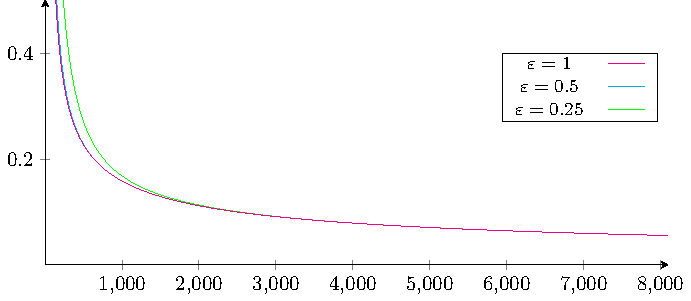
\includegraphics[]{"./proofs/fig6.pdf"}
    \caption{Graphe de la borne obtenue [\ref{EDE}] en fonction de \(n\) pour \(\rho = 1/\sqrt n\).}
\end{figure}





\section{Comparaison entre le mécanisme de sensibilité inverse et la méthode des histogrammes}


Dans les sections précédentes nous avons présenté la méthode de sensibilité inverse ainsi que la méthode que nous avons introduite, la méthode des histogrammes. Nous avons étudié en détail notre méthode et nous avons reporté une partie de l'étude du mécanisme de sensibilité inverse et nous avons produit des résultats supplémentaires. Ces deux méthodes présentent de bonnes bornes de précisions tout en étant \(\varepsilon\)-differentially private.\\

Pour cette comparaison nous avons décidé de nous concentrer sur deux aspects principaux aspects: la précisions des algorithmes pour des lois usuelles et l'influence du choix de \(\varepsilon\) sur la précision avec des données réelles. Les lois usuelles étudiées sont la loi uniforme sur \([0,1]\) et la loi normale centrée réduite. Nous avons choisis ces deux lois car elles modélisent de nombreux phénomènes courants et que les lois normales ont une importance particulière en statistique grâce au théorème central limite.

\subsection{Comparaison des bornes obtenues}

\subsection{Résultats expérimentaux}
\subsubsection{Le cas de la loi uniforme standard}

% Rappelons déjà que la loi uniforme standard représente toute les lois uniformes sur \(\R\). En effet, toutes les lois uniformes peuvent être transformées en la loi normale standard par simple application d'un isomorphisme réel.

Nous avons calculé l'écart quadratique moyen en fonction de la taille de l'échantillon dans le cas de la loi uniforme standard. Pour cela, pour tout \(n \in \inte 100 5000 \) nous avons lancé les deux algorithmes sur 50 ensembles de données indépendants et identiquement distribué suivant \(\mathcal U(0,1)\). \\ 

\begin{figure}[H]
    \centering
    \subfloat[\(\varepsilon = 0.5\)]{\centering 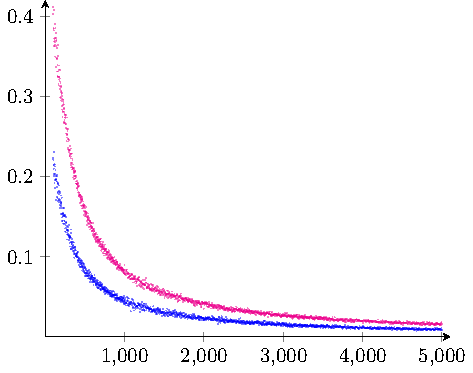
\includegraphics[width=.3\textwidth]{"./proofs/fig3_0.500000.pdf"}}
    \hfill
    \subfloat[\(\varepsilon = 1\)]{\centering 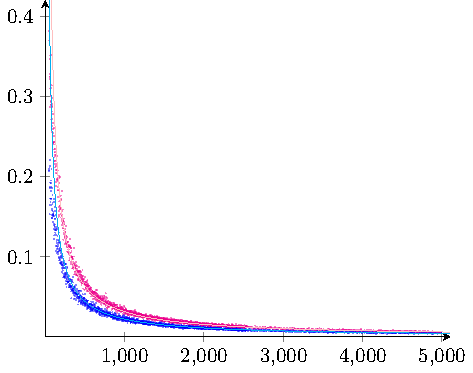
\includegraphics[width=.3\textwidth]{"./proofs/fig3_1.000000.pdf"}}
    \hfill
    \subfloat[\(\log-\log\) : \(\varepsilon = 1\)]{\centering 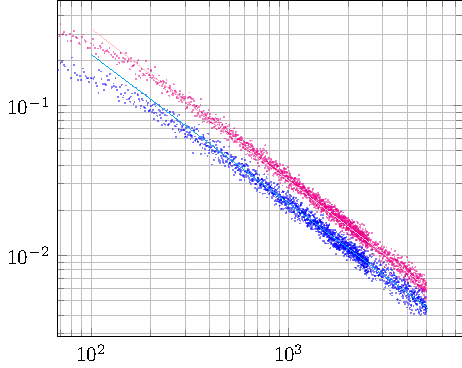
\includegraphics[width=.3\textwidth]{"./proofs/fig3_1.000000_log_log.pdf"}}
    \caption{Écart-quadratique moyen sur le calcul des déciles en fonction de \(n\) (la taille de l'échantillon). La méthode des histogrammes est en {\color{magenta} magenta} et le mécanisme de sensibilité inverse est en {\color{blue} bleu}.}
\end{figure}

Le graphe \(\log-\log\) montre que dans le cas \(\varepsilon = 1\), l'écart quadratique semble être d’espérance \(\color{magenta} 35n^{-1.015}\) pour la méthode des histogrammes et \(\color{blue} 21.5n^{-0.995}\) pour le mécanisme de sensibilité inverse. On observe alors que pour des valeurs de \(n\) courantes (\(\leq 10^8\)), le mécanisme de sensibilité inverse semble meilleur que la méthode que nous avons introduite et que \textbf{notre méthode est asymptotiquement meilleure} même si cela ne sera pas le cas en pratique.\\

Enfin, les deux mécanismes offrent vraiment des performances similaires. Le mécanisme de sensibilité inverse devrait être privilégié pour obtenir une meilleure précision. Néanmoins, la méthode des histogrammes est une alternative viable.

\subsubsection{La loi normale centrée réduite}


Nous avons suivi la même méthodologie que dans le cas de la loi uniforme standard. Les résultats obtenues sont similaires. les résultats suivent moins uniformément le modèle d'une puissance mais semble aussi y coller. Comme dans le cas uniforme, l'écart quadratique est moins bon avec la méthode des histogrammes. Néanmoins, cet écart semble asymptotiquement meilleur par rapport à celui obtenue avec le mécanisme de sensibilité inverse. 

\begin{figure}[H]
    \centering
    \subfloat[\(\varepsilon = 0.5\)]{\centering 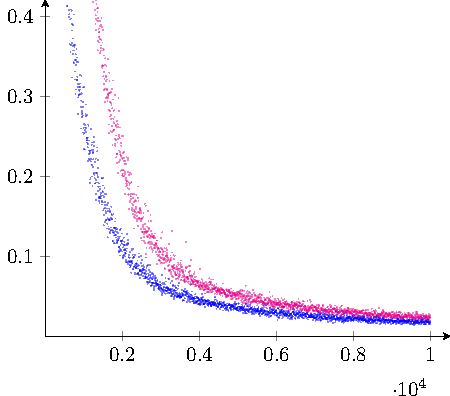
\includegraphics[width=.3\textwidth]{"./proofs/fig4_0.500000.pdf"}}
    \hfill
    \subfloat[\(\varepsilon = 1\)]{\centering 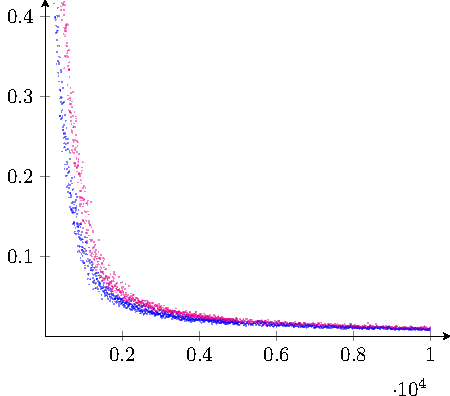
\includegraphics[width=.3\textwidth]{"./proofs/fig4_1.000000.pdf"}}
    \hfill
    \subfloat[\(\log-\log\) : \(\varepsilon = 1\)]{\centering 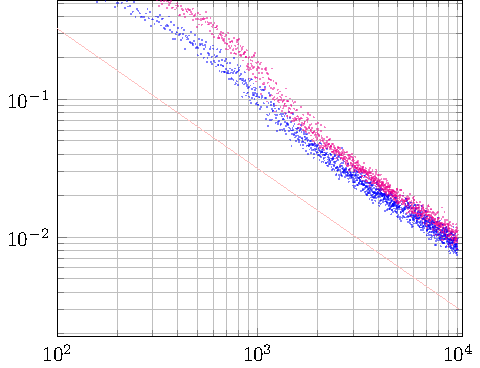
\includegraphics[width=.3\textwidth]{"./proofs/fig4_1.000000_log_log.pdf"}}
    \caption{Écart-quadratique moyen sur le calcul des déciles en fonction de \(n\) (la taille de l'échantillon). La méthode des histogrammes est en {\color{magenta} magenta} et le mécanisme de sensibilité inverse est en {\color{blue} bleu}.}
\end{figure}




\subsubsection{Des données réelles}

\begin{wrapfigure}{l}{.35\textwidth}
    \centering
    % \includegraphics[trim={5cm 10cm 12cm 10cm}, clip, width=.5\textwidth]{representation.png}
    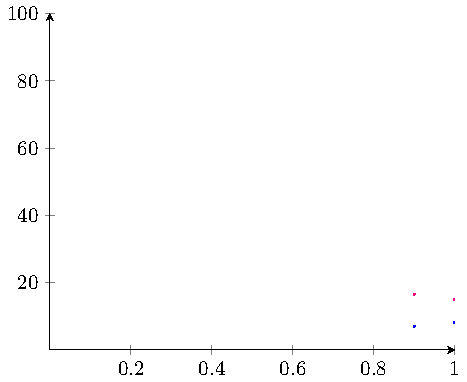
\includegraphics[width=0.35\textwidth, clip]{"./proofs/fig2.pdf"}
    \caption{Écart-quadratique sur le calcul des déciles en fonction de \(\varepsilon\). La méthode des histogrammes est en {\color{magenta} magenta} et le mécanisme de sensibilité inverse est en {\color{blue} bleu}.}
    \label{fig2}
\end{wrapfigure}

{Nous avons décidé de comparer les résultats des deux méthodes sur une base de donnée réelle \cite{salaries} afin de voir comment les méthodes se comportent vraiment en pratique. Pour cela nous avons utilisé les salaires annuels des agents du publique de l'état de New-York (États-Unis). Ces données ont directement été publiques par une agence gouvernementale, ce qui assure une certaine fiabilité. Nous travaillons alors sur un ensemble de près de 400 000 salaires annuels.\\

Les courbes sur le graphe \ref{fig2} sont des SMA\(_{10}\) (\textit{simple moving average} de paramètre 10). Cet indicateur permet de lisser les fluctuations locales afin de mettre en avant les tendances globales. Ainsi, le graphe \ref{fig2} montre que la méthode de sensibilité inverse est globalement plus précise. Il n'y a toute fois pas d'ordre de grandeur de différence entre les erreurs de deux algorithmes. Leurs performances sont donc similaires.\\

De plus, ces deux algorithmes fournissent des résultats précis. En effet, les déciles du jeu de donné sont 34 902, 38 574, 41 848, 46 862, 56 844, 67 121, 75 254, 84 751 et 99 637. L'erreur quadratique observée, proche de 20 est donc négligeable au vu des ordres de grandeurs des données.}



\newpage
\cleardoublepage
\phantomsection
\addcontentsline{toc}{section}{Références}
\printbibliography





\newpage
\pagenumbering{roman}
\appendix

\section{Démonstration de théorèmes utiles}

\subsection{Loi des statistiques d'ordre}\label{statordre}

TODO

\subsection{Inégalité d'{\sc Hoeffding}}\label{hoef}

TODO

\subsection{Bornes multiplicatives de {sc Chernoff}}\label{chern}

TODO

\subsection{Déciles de la loi normale centrée réduite}

TODO

\section{Le mécanisme de sensibilité inverse - probabilité de précision sur les déciles empiriques}\label{SI_empi}


\theoreme{}\\
Soit \(\gamma \in \R_+^\star\), \(u \in [0, \gamma/4]\), \(\rho \in \R_+\) et \(X \in [0,R]^n\) dont les éléments sont obtenues à partir d'une loi \(P\) de densité \(\pi_P\) continue au voisinage de ses déciles. On pose \(p_{\text{min}, i} = \inf_{t \in [d_i^l - 2\gamma, d_i^l + 2\gamma]} \pi_P(t)\). On note \((d_i)_i\) les déciles empirique de \(X\) et \((d_i^l)_i\) les déciles de la loi. Notons alors enfin \(M_{\text{cont}}\) le mécanisme de sensibilité inverse \(\rho\)-lisse.
\[
    \mathbb P\left( |M_{\text{cont}, i} - d_i| > 2u + \rho\right) \leq \dfrac{R}{2\rho}\exp\left(- \dfrac{np_{\text{min}, i}u\varepsilon}{4} \right) + 4\exp\left(- \dfrac{n\gamma^2p_{\text{min},i}^2}{8} \right) + \dfrac{2\gamma}{u}\exp\left( -\dfrac{np_{\text{min},i}u}{8} \right)
\]


\textit{démonstration:} Ce théorème donne une borne exponentielle sur la précision de l'algorithme. Le démonstration est longue.\\

Découpons l'intervalle \([d_i^l - \gamma, d_i^l + \gamma]\) en intervalles \((I_j)_j\) de taille \(u\). Pour tout \(j\), on pose \(N_j = \#I_j\). On note alors \(A\) l'événement ``pour tout \(j\), \(N_j \geq nup_{\text{min}, i}/2\)'' et \(B_i\) l'événement ``\(|d_i^l - d_i| \geq \gamma/2\)''.\\
\begin{align*}
    \mathbb P\left( |M_{\text{cont}, i} - d_i^l| > 2u + \rho \right) & = \mathbb P\left( |M_{\text{cont}, i} - d_i^l| > 2u + \rho \ | \ A \wedge B_i\right)\mathbb P\left( A \wedge B_i \right)\\
    & \quad \quad  + \mathbb P\left( |M_{\text{cont}, i} - d_i^l| > 2u + \rho \ | \ \overline A \vee \overline B_i\right) \mathbb P \left( \overline A \vee \overline B_i \right)\\
    & \leq \mathbb P\left( |M_{\text{cont}, i} - d_i^l| > 2u + \rho \ | \ A \wedge B_i\right) +   \mathbb P \left( \overline A \vee \overline B_i \right)\\
    & = \mathbb P\left( |M_{\text{cont}, i} - d_i^l| > 2u + \rho \ | \ A \wedge B_i\right) +   \mathbb P \left( (\overline A \wedge B_i) \vee \overline B_i \right)\\
    & \leq \mathbb P\left( |M_{\text{cont}, i} - d_i^l| > 2u + \rho \ | \ A \wedge B_i\right) +   \mathbb P \left( \overline A \wedge B_i\right) + \mathbb P \left( \overline B_i \right)\\
    & = \mathbb P\left( |M_{\text{cont}, i} - d_i^l| > 2u + \rho \ | \ A \wedge B_i\right) +   \mathbb P \left( \overline A \ |\ B_i\right)\mathbb P (B_i) + \mathbb P \left( \overline B_i \right)\\
    & \leq \mathbb P\left( |M_{\text{cont}, i} - d_i^l| > 2u + \rho \ | \ A \wedge B_i\right) +   \mathbb P \left( \overline A \ |\ B_i\right) + \mathbb P \left( \overline B_i \right)\\
\end{align*}

Nous savons que si les événements \(A\) et \(B\) surviennent, pour tout \(t\) tel que \(|t - d_i| > 2u\), au moins \(nup_{\text{min}, i}/2\) éléments séparent \(d_i\) et \(t\). Pour de tels \(t\) nous avons alors \(\len_f(x,t) \geq nup_{\text{min}, i}/2\). Ainsi, pour tout \(s\) tel que \(|s - d_i| > 2u + \rho\), \(\len_f^\rho(x,s) \geq nup_{\text{min}, i}/2\). Enfin, pour tout \(t\) tel que \(|t - d_i| > 2u + \rho\),
\begin{align*}
    \pi_P\left( t\ |\ A \wedge B \right) & = \dfrac{\exp\left( -{\len_f^\rho(x,t)\varepsilon}/{2} \right)}{\int_\mathcal T \exp\left( {-\len_f^\rho(x,s)\varepsilon}/{2} \right)\dt \mu(s)}\\
    & \leq \dfrac{\exp\left( -{nup_{\text{min}, i}\varepsilon}/{4} \right)}{\int_\mathcal T \exp\left( {-\len_f^\rho(x,s)\varepsilon}/{2} \right)\dt \mu(s)}\\
    & \leq \dfrac{\exp\left( -{nup_{\text{min}, i}\varepsilon}/{4} \right)}{\int_{d_i-\rho}^{d_i+\rho} \exp\left( {-\len_f^\rho(x,s)\varepsilon}/{2} \right)\dt \mu(s)}\\
    & = \dfrac{\exp\left( -{nup_{\text{min}, i}\varepsilon}/{4} \right)}{\int_{d_i-\rho}^{d_i+\rho}\dt \mu(s)}\\
    & = \dfrac{\exp\left( -{nup_{\text{min}, i}\varepsilon}/{4} \right)}{2\rho}\\
\end{align*}

Ainsi,
\begin{align*}
    \mathbb P\left( |M_{\text{cont}} - d_i| > 2u + \rho \ | \ A \wedge B_i\right) & \leq \int_\mathcal T \dfrac{\exp\left( -{nup_{\text{min}, i}\varepsilon}/{4} \right)}{2\rho}\un_{| t - d_i| > 2u + \rho} \dt\mu(t)\\
    & \leq \dfrac{\exp\left( -{nup_{\text{min}, i}\varepsilon}/{4} \right)}{2\rho} \mu(\mathcal T)\\
    & = \dfrac{R}{2\rho}\exp\left( -{nup_{\text{min}, i}\varepsilon}/{4} \right)
\end{align*}

Nous allons maintenant calculer la probabilité de l'événement \(\overline B_i\). Pour cela, on pose \(\alpha = \gamma/2\), pour tout \(j \in \inte 0 {n-1} \) on pose \(C_j^i = \un_{x_i > d_i^l + \alpha}\) et \(C^i = \sum_{j = 0}^{n-1} C_j\). L'événement \(C^i\) dénote le nombre d'éléments de \(X\) plus grands que \(d_i^l + \alpha\). Par définition de \(p_{\text{min}, i}\) assure que 
\[
    \begin{array}{rcl}
        \hat p & := & \mathbb P(C_j^i = 1)\\
        & = & 1 - \displaystyle\int_{0}^{d_i^l} \pi_P(t) \dt \mu(t) - \displaystyle \int_{d_i^l}^{d_i^l+\alpha} \pi_P(t) \dt \mu(t)\\
        & \overset{\text{déf de } d_i^l}{=} & 1 - \dfrac{i}{10} - \displaystyle\int_{d_i^l}^{d_i^l+\alpha} \pi_P(t) \dt \mu(t)\\
        & \leq & \dfrac{10 - i}{10} - \displaystyle p_{\text{min}, i}\int_{d_i}^{d_i^l+\alpha} \dt \mu(t)\\
        & = & \dfrac{10-i}{10} - \alpha p_{\text{min}, i}\\
    \end{array}
\]

Or, si \(d_i > d_i^l\), \(C^i \geq in/10\). Ainsi, en utilisant une borne de {\sc Chernoff} (démontré en annexe [\ref{chern}]) (\(C^i\) est d'espérance \(\hat pn\) et les \((C^i_j)_j\) sont indépendantes),
\begin{align*}
    \mathbb P\left( d_i > d_i^l + \alpha \right)& \leq \mathbb P \left( C^i \geq \dfrac{in}{10}\right)\\
    % & = \mathbb P \left( \sum_{j = 0}^{n-1}C^i_j \geq \hat pn\left( 1 + \dfrac{i}{\hat p 10} -1\right)\right)\\
    & = \mathbb P \left( \sum_{j = 0}^{n-1}C^i_j \geq \hat pn\left( 1 - \left(1 - \dfrac{i}{\hat p 10}\right)\right)\right)\\
    & \leq \exp\left( -\left(1 - \dfrac{i}{\hat p 10}\right)^2\dfrac{n\hat p}{2}\right)\\
    & = \exp\left( -\left(\hat p - \dfrac{i}{10}\right)^2\dfrac{n}{2\hat p}\right)\\
    & \leq \exp\left( -\left(\alpha p_{\text{min}, i}\right)^2\dfrac{n}{2\hat p}\right)\\
    & \leq \exp\left( -\alpha^2 p_{\text{min}, i}^2\dfrac{n}{i/5 - 2\alpha p_{\text{min}, i}}\right)\\
    & \leq \exp\left( -\dfrac{1}{2}\alpha^2 p_{\text{min}, i}^2n\right)\\
\end{align*}

On montre alors de même que \(\mathbb P\left( d_i < d_i^l - \alpha \right) < \exp\left( -\dfrac{1}{2}\alpha^2 p_{\text{min}, i}^2n\right)\). Nous avons donc montré que 
\[
    \mathbb P \left( B_i \right) \geq 1 - 2\exp\left( -\dfrac{1}{8}n\gamma^2 p_{\text{min}, i}^2\right)
\]

Finalement, il ne nous reste plus qu'à minorer \(\mathbb P (A\ | \ B_i)\)! Pour cela, notons que 
\[
    \mathbb P (A\ | \ B_i) \geq (A\ | \ B_i)\mathbb P(B_i) = \mathbb P (A) - \mathbb P \left( A \wedge \overline B_i \right) \geq \mathbb P (A) - \mathbb P (\overline B_i)
\]

Pour tout \(k \leq n - 1\) on pose alors \(Z_k = \un_{x_k \in I_j}\) et on a \(N_j = \sum_{k = 0}^{n-1} Z_k\). On note que \(\mathbb P (Z_j = 1) \geq u p_{\text{min}, i}\). Utiliser une nouvelle fois une borne de {\sc Chernoff} (démontré en annexe [\ref{chern}]) assure enfin que 
\[
    \mathbb P \left( N_j < n u p_{\text{min}, i}/2\right) = \mathbb P \left( N_j < n u p_{\text{min}, i} \left( 1 - \dfrac{1}{2} \right)\right) < \exp\left( - \dfrac{1}{8}n u p_{\text{min}, i} \right)
\]

Enfin,
\[
  \mathbb P \left( \overline A \right)  = \mathbb P \left( \bigcup_{j = 0}^{2\gamma /u} N_j < n u p_{\text{min}, i}/2  \right) \leq \sum_{j = 0}^{2\gamma/u} \mathbb P \left( N_j < n u p_{\text{min}, i}/2 \right) \leq \dfrac{2\gamma}{u}\exp\left( - \dfrac{1}{8}n u p_{\text{min}, i} \right)
\]


On obtient alors 
\[
    \mathbb P (A\ | \ B_i) \geq 1 - \dfrac{2\gamma}{u}\exp\left( - \dfrac{1}{8}n u p_{\text{min}, i} \right) - 2\exp\left( -\dfrac{1}{8}n\gamma^2 p_{\text{min}, i}^2\right) 
\]

Ce que nous permet alors d'obtenir le résultat recherché!


\section{HistogramMethod: Analyse de précision - le cas de la loi normale centrée réduite}
\label{hmncr}
% \subsection{Démonstration du lemme [\ref{ecard_deciles_empirique_loi_n01}]}

\lemme{Estimation de l'écard entre les déciles empiriques et ceux de la loi normale centrée réduite.}\\
Soit \(X\) un ensemble de \(n\) variables aléatoires \((X_i)_i\) indépendantes et suivant toutes la loi normale centrée réduite et soit \(\gamma \in [0, d_i^l]\). Notons \((d_i)_i\) les déciles empiriques de \(X\) et \((d_i^l)_i\) les déciles de la loi normale centrée réduite. Pour tout \(i \in \inte 1 9\)
\[
    \mathbb P(d_i \in [d_i^l - \gamma/2, d_i^l + \gamma/2]) \geq 1 - \eta
\]
Avec 
\begin{align*}
    \eta & = \exp\left( - \dfrac{n\gamma^2}{i^2} \left( \dfrac{i}{10} - \dfrac{\gamma}{2\sqrt{2\pi}}\right)\exp\left( - (d_i^l)^2\right)\right) + \exp \left( - \dfrac{5 \gamma^2in}{16\pi \left( i + 5\gamma/\sqrt{2\pi} \right)^2}\exp\left( -(d_i^l)^2\right)  \right)
\end{align*}

\textit{Démonstration:} Soit \(X\) un ensemble de \(n\) variables aléatoires \((X_i)_i\) indépendantes et suivant toutes la loi uniforme sur [0,1]. Notons \((d_i)_i\) les déciles empiriques de \(X\) et \((d_i^l)_i\) ceux de la loi. Soit \(\gamma \in [0,d^l_i]\). On note que
\begin{align*}
    \mathbb P(d_i \in [d^l_i - \gamma/2, d^l_i + \gamma+2]) & = 1 - \mathbb P(d_i \notin [d^l_i - \gamma/2, d^l_i + \gamma/2])\\
    & = 1 - \mathbb P(d_i \leq d^l_i - \gamma/2 \vee d_i \geq d^l_i + \gamma/2)\\
\end{align*}

On pose alors \(A = \) ``il y a au moins \(in/10\) valeurs plus petites que \(d^l_i - \gamma/2\)'' et \(B = \) ``il y a au plus \(in/10\) valeurs plus petites que \(d^l_i + \gamma/2\)''. Pour tout \(j \in \inte 0 {n-1}\) on pose \(A_j = \un_{x_j \leq d^l_i + \gamma/2}\), \(B_j = \un_{x_j \leq d^l_i + \gamma/2}\), \(A_s = \sum_{j = 0}^{n-1} A_j\) et \(B_s = \sum_{j = 0}^{n-1}B_j\). On a alors, \(A = \{A_s \geq in/10\}\) et \(B = \{B_s \leq  in/10\}\). Une application d'une borne de {\sc Chernoff} (démontré en annexe [\ref{chern}]) assure alors que 
\[
    \begin{array}{rcl}
        \mathbb P(A) & = & \mathbb P (A_s \geq in/10)\\
        & = & \mathbb P \left(A_s \geq \dfrac{n}{\sqrt{2\pi}}\displaystyle\int_{-\infty}^{d^l_i - \gamma/2}   \exp\left( \dfrac{-t^2}{2} \right)\dt t  \left( 1 + \dfrac{i\sqrt{2\pi}}{10\int_{-\infty}^{d^l_i - \gamma/2}   \exp\left( {-t^2}/{2} \right)\dt t}  - 1\right)\right)\\
        & \overset{d_i ^l \geq \gamma}{\leq} & \exp\left( - \dfrac{n}{3\sqrt{2\pi}}\displaystyle\int_{-\infty}^{d^l_i - \gamma/2}   \exp\left( \dfrac{-t^2}{2} \right)\dt t\left( \dfrac{i\sqrt{2\pi}}{10\int_{-\infty}^{d^l_i - \gamma/2}   \exp\left( {-t^2}/{2} \right)\dt t}  - 1 \right)^2\right)\\
        & = & \exp\left( - \dfrac{n}{3} \left( \dfrac{i}{10} - \dfrac{1}{\sqrt{2\pi}}\displaystyle\int_{d^l_i - \gamma/2}^{d_i^l}  \exp\left( \dfrac{-t^2}{2} \right)\dt t \right)\left( \dfrac{i\sqrt{2\pi}}{10\int_{-\infty}^{d^l_i - \gamma/2}   \exp\left( {-t^2}/{2} \right)\dt t}  - 1 \right)^2\right)\\
        & \leq & \exp\left( - \dfrac{n}{3} \left( \dfrac{i}{10} - \dfrac{\gamma}{2\sqrt{2\pi}}\right)\left( \dfrac{i\sqrt{2\pi}}{10\int_{-\infty}^{d^l_i - \gamma/2}   \exp\left( {-t^2}/{2} \right)\dt t}  - 1 \right)^2\right)
    \end{array}
\]


Or, la valeurs des déciles de la loi normale centrée réduite étant connues \ref{val_deciles_n01},
\begin{align*}
    \dfrac{1}{\sqrt{2\pi}} \int_{-\infty}^{d^l_i - \gamma/2}   \exp\left( \dfrac{-t^2}{2} \right)\dt t & = \dfrac{1}{2}\dfrac{2}{\sqrt{\pi}}  \int_{-\infty}^{(d^l_i - \gamma/2)/\sqrt 2}   \exp\left( {-t^2} \right)\dt t\\
    & = \dfrac{1}{2} + \dfrac{1}{2}\erf\left( \dfrac{d^l_i - \gamma/2}{\sqrt 2 }\right)\\
    & = \dfrac{1}{2} + \dfrac{1}{2}\erf\left( \erf^{-1}\left( 2\times 0.1i - 1 \right) - \dfrac{\gamma}{2\sqrt 2 }\right)\\
    & = \dfrac{1}{2} + \dfrac{1}{2}\erf\left( \erf^{-1}\left( 2\times 0.1i - 1 \right)\right) - \dfrac{1}{\sqrt{\pi}}\int_{\erf^{-1}\left( 2\times 0.1i - 1 \right) - \gamma/2\sqrt 2}^{\erf^{-1}\left( 2\times 0.1i - 1 \right)} \exp\left( -t^2 \right)\dt t\\
    & = \dfrac{i}{10} - \dfrac{1}{\sqrt{\pi}}\int_{\erf^{-1}\left( 2\times 0.1i - 1 \right) - \gamma/2\sqrt 2}^{\erf^{-1}\left( 2\times 0.1i - 1 \right)} \exp\left( -t^2 \right)\dt t\\
    & \leq \dfrac{i}{10} - \dfrac{\gamma}{2\sqrt{2\pi}} \exp\left( - \erf^{-1}\left(2\times 0.1i - 1 \right)^2\right) \\
\end{align*}

Enfin, comme \(25/(6\pi) \geq 5\),
\begin{align*}
    \mathbb P(A) & \leq \exp\left( - \dfrac{n}{3} \left( \dfrac{i}{10} - \dfrac{\gamma}{2\sqrt{2\pi}}\right)\left( \dfrac{i}{i - {5\gamma}/{\sqrt{2\pi}} \exp\left( - \erf^{-1}\left(2\times 0.1i - 1 \right)^2\right)}  - 1 \right)^2\right)\\
    & \leq \exp\left( - \dfrac{n\gamma^2}{i^2} \left( \dfrac{i}{10} - \dfrac{\gamma}{2\sqrt{2\pi}}\right)\exp\left( - 2\erf^{-1}\left(2\times 0.1i - 1 \right)^2\right)\right)\\
    & = \exp\left( - \dfrac{n\gamma^2}{i^2} \left( \dfrac{i}{10} - \dfrac{\gamma}{2\sqrt{2\pi}}\right)\exp\left( - (d_i^l)^2\right)\right)
\end{align*}

Finalement,
\begin{align*}
    \mathbb P (B) & = \mathbb P \left( B_s \leq in/10 \right)\\
    &= \mathbb P\left( B_s \leq \dfrac{n}{\sqrt{2\pi}}\left( \int_{-\infty}^{d_i^l + \gamma/2} \exp\left( -\dfrac{t^2}{2}\dt t \right) \right)\left( 1 - \left( 1 - \dfrac{i\sqrt{2\pi}}{10\int_{-\infty}^{d_i^l + \gamma/2} \exp\left( -{t^2}/{2} \right)\dt t}  \right)\right)  \right)\\
    & \leq \exp \left( - \dfrac{n}{2\sqrt{2\pi}}\left( \int_{-\infty}^{d_i^l + \gamma/2} \exp\left( -\dfrac{t^2}{2}\dt t \right) \right)\left( 1 - \dfrac{i\sqrt{2\pi}}{10\int_{-\infty}^{d_i^l + \gamma/2} \exp\left( -{t^2}/{2} \right)\dt t}  \right)^2  \right)\\
    & \leq \exp \left( - \dfrac{in}{20}\left( 1 - \dfrac{i}{i + 5\gamma/\sqrt{2\pi} \exp\left( -(\erf^{-1}\left(2\times 0.1i - 1 \right) + \gamma/2) ^2\right)}  \right)^2  \right)\\
    &  = \exp \left( - \dfrac{25 \gamma^2in}{40\pi}\left(\dfrac{\exp\left( -(\erf^{-1}\left(2\times 0.1i - 1 \right) + \gamma/2)^2\right)}{i + 5\gamma/\sqrt{2\pi} \exp\left( -(d_i^l + \gamma/2)^2\right)}  \right)^2  \right)\\
    &  \leq \exp \left( - \dfrac{5 \gamma^2in}{16\pi \left( i + 5\gamma/\sqrt{2\pi} \right)^2}\exp\left( -2(\erf^{-1}\left(2\times 0.1i - 1 \right) + \gamma/2)^2\right)  \right)\\
    &  \leq \exp \left( - \dfrac{5 \gamma^2in}{16\pi \left( i + 5\gamma/\sqrt{2\pi} \right)^2}\exp\left( -(d_i^l)^2\right)  \right)\\
\end{align*}


% \subsection{Démonstration du lemme [\ref{ecard_deciles_empirique_loi_n02}]}
\lemme{}

Soit \(X\) un ensemble de \(n\) variables aléatoires \((X_i)_i\) indépendantes et suivant toutes la normale centrée réduite. Soit \(\gamma \in [0,d^l_i]\), \(i \in \inte 1 9 \) et \(k \in \N\). Il y a au moins \(\alpha\) valeurs de \(X\) dans chacun des intervalles \([d^l_i - \gamma, d^l_i-\gamma/2]\) et \([d^l_i + \gamma/2, d^l_i+\gamma]\) avec une probabilité au moins \(1 - \beta\) avec 
\begin{align*}
    \beta & = 2\exp\left( -\dfrac{n\gamma}{4\sqrt{2\pi}}  \left(\exp\left( -\dfrac{(|d_i^l| + \gamma)^2}{2} \right)  - \dfrac{2\alpha\sqrt{2\pi}}{n\gamma} \right)^3\right)
\end{align*}

\textit{Démonstration:} Soit \(X\) un ensemble de \(n\) variables aléatoires \((X_i)_i\) indépendantes et suivant toutes la loi normale centrée réduite. Soit \(\gamma \in [0,d^l_i]\), \(i \in \inte 1 9 \) et \(\alpha \in \N\). On pose \(A = \) ``il y a au moins \(\alpha\) valeurs dans l'intervalle \([d^l_i - \gamma, d_i^l - \gamma/2]\)'' et \(B = \) ``il y a au moins \(\alpha\) valeurs dans l'intervalle \([d^l_i + \gamma/2, d_i^l + \gamma]\)''. Pour tout \(j \in \inte 0 {n-1}\) on pose \(A_j = \un_{x_j \in [d^l_i - \gamma, d_i^l - \gamma/2]}\), \(B_j = \un_{x_j \in [d^l_i + \gamma/2, d_i^l + \gamma]}\), \(A_s = \sum_{j = 0}^{n-1} A_j\) et \(B_s = \sum_{j = 0}^{n-1}B_j\). On a alors, \(A = \{A_s \geq \alpha\}\) et \(B = \{B_s \geq  \alpha\}\).
\begin{align*}
    \mathbb P \left( A\ \wedge\ B \right) &= \mathbb P\left( A_s \geq \alpha \ \wedge \ B_s \geq \alpha \right)\\
    & \geq \mathbb P\left( A_s \geq \alpha \right) + \mathbb P \left(B_s \geq \alpha \right) - 1\\
    & = 1 - \mathbb P\left( A_s < \alpha \right) - \mathbb P \left(B_s < \alpha \right)\\
\end{align*}

Une application d'une borne de {\sc Chernoff} (démontré en annexe [\ref{chern}]) assure alors que 
\begin{align*}
    \mathbb P\left( A_s < \alpha \right) & = \mathbb P\left( A_s < \dfrac{n}{\sqrt{2\pi}}\int_{d^l_i - \gamma}^{d^l_i - \gamma/2} \exp\left( -\dfrac{t^2}{2} \right)\dt t \left( 1 - \left(1 - \dfrac{\alpha\sqrt{2\pi}}{n \int_{d^l_i - \gamma}^{d^l_i - \gamma/2} \exp\left( -{t^2}/{2} \right)\dt t} \right) \right)\right) \\
    & \leq \exp\left( -\dfrac{n}{2\sqrt{2\pi}}\int_{d^l_i - \gamma}^{d^l_i - \gamma/2} \exp\left( -\dfrac{t^2}{2} \right)\dt t  \left(1 - \dfrac{\alpha\sqrt{2\pi}}{n \int_{d^l_i - \gamma}^{d^l_i - \gamma/2} \exp\left( -{t^2}/{2} \right)\dt t} \right)^2\right)\\
    & \leq \exp\left( -\dfrac{n\gamma}{4\sqrt{2\pi}} \exp\left( -\dfrac{(|d_i^l| + \gamma)^2}{2} \right)  \left(\dfrac{n \int_{d^l_i - \gamma}^{d^l_i - \gamma/2} \exp\left( -{t^2}/{2} \right)\dt t - \alpha\sqrt{2\pi}}{n \int_{d^l_i - \gamma}^{d^l_i - \gamma/2} \exp\left( -{t^2}/{2} \right)\dt t} \right)^2\right)\\
    & \leq \exp\left( -\dfrac{1}{n\gamma\sqrt{2\pi}} \exp\left( -\dfrac{(|d_i^l| + \gamma)^2}{2} \right)  \left(n \int_{d^l_i - \gamma}^{d^l_i - \gamma/2} \exp\left( -{t^2}/{2} \right)\dt t - \alpha\sqrt{2\pi} \right)^2\right)\\
    & \leq \exp\left( -\dfrac{n}{\gamma\sqrt{2\pi}} \exp\left( -\dfrac{(|d_i^l| + \gamma)^2}{2} \right)  \left( \dfrac{\gamma}{2}\exp\left( -\dfrac{(|d_i^l| + \gamma)^2}{2} \right)  - \dfrac{\alpha\sqrt{2\pi}}{n} \right)^2\right)\\
    & \leq \exp\left( -\dfrac{n\gamma}{4\sqrt{2\pi}}  \left(\exp\left( -\dfrac{(|d_i^l| + \gamma)^2}{2} \right)  - \dfrac{2\alpha\sqrt{2\pi}}{n\gamma} \right)^3\right)\\
\end{align*}

Nous pourrions alors montrer, exactement de la même manière que 
\begin{align*}
    \mathbb P\left( B_s < \alpha \right) & \leq \exp\left( -\dfrac{n\gamma}{4\sqrt{2\pi}}  \left(\exp\left( -\dfrac{(|d_i^l| + \gamma)^2}{2} \right)  - \dfrac{2\alpha\sqrt{2\pi}}{n\gamma} \right)^3\right)\\
\end{align*}

Finalement,
\[
    \mathbb P \left( A\ \wedge\ B \right) \geq 1 - 2\exp\left( -\dfrac{n\gamma}{4\sqrt{2\pi}}  \left(\exp\left( -\dfrac{(|d_i^l| + \gamma)^2}{2} \right)  - \dfrac{2\alpha\sqrt{2\pi}}{n\gamma} \right)^3\right)
\]

% \subsection{Démonstration du théorème [\ref{ecard_deciles_empirique_loi_n03}]}

\theoreme{\((\alpha, \beta)\)-précision de \mintinline{cpp}{HistogramMethod} dans le cas de la loi normale centrée réduite}

Soit \(X\) un ensemble de \(n\) variables aléatoires \((X_i)_i\) indépendantes et suivant toutes la loi normale centrée réduite. Soit \(\gamma \in [0,d_i^l]\), \(i \in \inte 1 9 \), \(k \in \N\) et \(\beta \in [0,1]\). Notons \((d_i)_i\) les déciles empiriques de \(X\) et \((d_i^l)_i\) les déciles de la loi normale centrée réduite. Posons \(A\) la variable aléatoire \mintinline{cpp}{HistogramMethod(X, epsilon, k, a, b)}.

\[
    \mathbb P\left( A_i \in [d_i^l-\gamma, d_i^l + \gamma] \right) \geq 1 - \beta - \eta -\mu    
\]
Avec 
\[
    \left\{ 
        \begin{array}{rl}
            \alpha & = \dfrac{8\left( \log k + \log(2/\beta) \right)}{\varepsilon} \\
            \mu & = 2\exp\left( -\dfrac{n\gamma}{4\sqrt{2\pi}}  \left(\exp\left( -\dfrac{(|d_i^l| + \gamma)^2}{2} \right)  - \dfrac{2\alpha\sqrt{2\pi}}{n\gamma} \right)^3\right)\\
            \eta & = \exp\left( - \dfrac{n\gamma^2}{i^2} \left( \dfrac{i}{10} - \dfrac{\gamma}{2\sqrt{2\pi}}\right)\exp\left( - (d_i^l)^2\right)\right) + \exp \left( - \dfrac{5 \gamma^2in}{16\pi \left( i + 5\gamma/\sqrt{2\pi} \right)^2}\exp\left( -(d_i^l)^2\right)  \right)\\
        \end{array}
    \right.     
\] 

\textit{Démonstration:} Soit \(X\) un ensemble de \(n\) variables aléatoires \((X_i)_i\) indépendantes et suivant toutes la loi normale centrée réduite. Soit \(\gamma \in [0,d_i^l]\), \(i \in \inte 1 9 \), \(k \in \N\) et \(\beta \in [0,1]\). Notons \((d_i)_i\) les déciles empiriques de \(X\) et \((d_i^l)_i\) les déciles de la loi normale centrée réduite. Posons \(A\) la variable aléatoire \mintinline{cpp}{HistogramMethod(X, epsilon, k, a, b)}.\\

On pose 
\[
    \alpha = \dfrac{8\left( \log k + \log(2/\beta) \right)}{\varepsilon}    
\]

Notons alors \(E_\alpha\) l'événement ``Il y a au moins \(\alpha\) valeurs de \(X\) dans chacun des intervalles \([d_i^l - \gamma, d_i^l-\gamma/2]\) et \([d_i^l + \gamma/2, d_i^l+\gamma]\)'' Et \(E_{A_i}\) l'événement ``moins de \(\alpha\) valeurs de \(X\) séparent \(d_i\) et \(A_i\)''. Nous avons alors 
\begin{align*}
    \mathbb P\left( A_i \in [d_i^l-\gamma, d_i^l + \gamma] \right) & \geq \mathbb P \left( E_{A_i} \wedge E_\alpha \wedge d_i \in [d_i^l - \gamma/2, d_i^l + \gamma/2]  \right)\\
    & \geq \mathbb P \left( E_{A_i}\right) + \mathbb P \left( E_\alpha\right) + \mathbb P \left( d_i \in [d_i^l - \gamma/2, d_i^l + \gamma/2]  \right) - 2\\
\end{align*}

Les lemmes précédent assurent alors que 
\begin{align*}
    \mathbb P\left( A_i \in [0.1i-\gamma, 0.1i + \gamma] \right) & \geq (1 - \beta) + (1 - \mu) + (1 - \eta) - 2\\
    & \geq 1 - \beta - \mu - \eta
\end{align*}

Avec 
\[
    \left\{ 
        \begin{array}{rl}
            \alpha & = \dfrac{8\left( \log k + \log(2/\beta) \right)}{\varepsilon} \\
            \mu & = 2\exp\left( -\dfrac{n\gamma}{4\sqrt{2\pi}}  \left(\exp\left( -\dfrac{(|d_i^l| + \gamma)^2}{2} \right)  - \dfrac{2\alpha\sqrt{2\pi}}{n\gamma} \right)^3\right)\\
            \eta & = \exp\left( - \dfrac{n\gamma^2}{i^2} \left( \dfrac{i}{10} - \dfrac{\gamma}{2\sqrt{2\pi}}\right)\exp\left( - (d_i^l)^2\right)\right) + \exp \left( - \dfrac{5 \gamma^2in}{16\pi \left( i + 5\gamma/\sqrt{2\pi} \right)^2}\exp\left( -(d_i^l)^2\right)  \right)\\
        \end{array}
    \right.    
\]

% \vspace{30px}
% \vspace{15px}


\end{document} 